\documentclass[11pt]{report}
\usepackage{graphics}
\usepackage{graphicx}
\usepackage{epsfig}
\usepackage{fancyhdr}
\usepackage{fullpage}
\usepackage{epsfig}
\usepackage{tabularx,ragged2e,booktabs,caption}
\usepackage{algorithm}
\usepackage{algpseudocode}
\newcommand{\Try}{\State \textbf{try}}
\newcommand{\Catch}[1]{\State \textbf{catch} (#1)}
\newcommand{\EndTry}{\State \textbf{end try}}
\usepackage{tocloft}
\usepackage{longtable} 
\usepackage{enumitem}
\usepackage[hidelinks]{hyperref}
\usepackage{amsmath}
\usepackage{amssymb}
\DeclareUnicodeCharacter{2248}{\ensuremath{\approx}}
\DeclareUnicodeCharacter{2264}{\ensuremath{\le}}
\DeclareUnicodeCharacter{2713}{\checkmark}

\usepackage{comment}


\newlength{\mylen}
\renewcommand{\cftfigpresnum}{\figurename\enspace}
\renewcommand{\cftfigaftersnum}{:}
\settowidth{\mylen}{\cftfigpresnum\cftfigaftersnum}
\addtolength{\cftfignumwidth}{\mylen}

\renewcommand{\cfttabpresnum}{\tablename\enspace}
\renewcommand{\cfttabaftersnum}{:}
\settowidth{\mylen}{\cfttabpresnum\cfttabaftersnum}
\addtolength{\cfttabnumwidth}{\mylen}
\setlength{\arrayrulewidth}{0.35mm} % Global thickness setting


\begin{document}
\renewcommand\bibname{References}

\pagestyle{fancy}
\fancyhead{}
\fancyfoot{}
\fancyfoot[c]{\thepage}
\fancyfoot[l]{Dept. of Computer Engineering, MEC, 2025}

\renewcommand{\chaptermark}[1]{\markboth{\thechapter.\ #1}{}}
\renewcommand{\headrulewidth}{0.1pt}

\makeatletter
\renewcommand{\headrule}{%
  {\if@fancyplain\let\headrulewidth\plainheadrulewidth\fi
   \hrule\@height\headrulewidth\@width\headwidth
   \vskip 24pt}%
}
\makeatother

\setlength{\headheight}{38pt}

\fancyhead[L]{%
\parbox[t]{0.55\textwidth}{\footnotesize
Hybrid Input Mental Health Chatbot with Contextual Memory}}

\fancyhead[R]{%
\parbox[t]{0.40\textwidth}{\raggedleft\footnotesize\nouppercase{\leftmark}}}



\begin{titlepage}
\begin{center}

\LARGE{\textbf{Hybrid Input Mental Health Chatbot with Contextual Memory}}\\
\vspace{0.6in}
\large{\textbf{CSD415 Project Phase II \\}}
\vspace{0.5in}

\begin{center}
\begin{tabular}{lll}
\Large \textbf{LMDL22CS204} & \Large \textbf{22CSB67} & \Large \textbf{Kalyani M Biju}\\
\Large \textbf{LMDL22CS205} & \Large \textbf{22CSB68} & \Large \textbf{Muhammed Yasin M A}\\
\Large \textbf{LMDL22CS207} & \Large \textbf{22CSB69} & \Large \textbf{Raeesa Sayed Muhammed}\\
\Large \textbf{LMDL22CS212} & \Large \textbf{22CSB70} & \Large \textbf{Sreejith O}\\
\end{tabular}
\end{center}

\vspace{0.20in}
\Large{\textbf{B. Tech Computer Science \& Engineering}}

\vspace{0.5in}
\begin{figure}[h]
\centering
\epsfig{width=1.3in, file=logo.jpg}
\end{figure}
\vspace{0.5in}

\textbf{
Department of Computer Engineering\\
Model Engineering College\\
Thrikkakara, Kochi 682021\\
Phone: +91.484.2575370\\
http://www.mec.ac.in \\
hodcs@mec.ac.in\\
\vspace{0.9in}
{\upshape October 2025}
}
\end{center}
\end{titlepage}




\begin{titlepage}
\begin{center}
\Large{\textbf{Model Engineering College Thrikkakara}}\\
\Large{\textbf{Department of Computer Engineering}}\\
\end{center}
\begin{figure}[h]
\begin{center}
\epsfig{width=1.2in, file=logo.jpg}
\end{center}
\end{figure}
\begin{center}
\Large{\textbf{C E R T I F I C A T E}}\\
\vspace{.1in}
\end{center}
This is to certify that, this report titled  \textbf{\textit{Hybrid Input Mental Health Chatbot with Contextual Memory}} is a bonafide record of the work done by
\vspace{0.3cm}


\begin{center}
\begin{tabular}{lll}
\Large \textbf{LMDL22CS204} & \Large \textbf{22CSB67} & \Large \textbf{KALYANI M BIJU}\\
\Large \textbf{LMDL22CS205} & \Large \textbf{22CSB68} & \Large \textbf{MUHAMMED YASIN M A}\\
\Large \textbf{LMDL22CS207} & \Large \textbf{22CSB69} & \Large \textbf{RAEESA SAYED MUHAMMED}\\
\Large \textbf{LMDL22CS212} & \Large \textbf{22CSB70} & \Large \textbf{SREEJITH O}\\
\end{tabular}
\end{center}

\vspace{0.3cm}

\begin{center}
Seventh Semester B. Tech. Computer Science \& Engineering
\end{center}
scholar, under our guidance and supervision, in partial fulfillment of the requirements for the award of the degree, B. Tech. Computer Science and Engineering of \textbf{APJ Abdul Kalam Technological University}.
\\

\begin{tabular}{p{0.4\textwidth}p{0.2\textwidth}p{0.4\textwidth}}
\textbf{Guide:} & & \textbf{Coordinator:} \\[0.6cm]
& & \\
 Meghna Raj M & & Dr. Priya S \\
Assistant Professor & &Professor \\
Computer Engineering & & Computer Engineering \\
\end{tabular} 
\\ \\
\begin{center}
\textbf{Head of Department:} \\
\vspace{1.3cm}
Dr. Binu V P \\
Professor \\
Computer Engineering
\end{center}


\end{titlepage}









\begin{titlepage}
\vspace{.25in}	
\begin{center}
\textbf{Acknowledgements}\\
\end{center}
\normalsize

This project would not have been possible without the kind support and help of many individuals. We would like to extend my sincere thanks to all of them.
  
First of all, We would like to thank our esteemed Principal, Prof. (Dr.) Mini M.G., for her guidance and support in maintaining a calm and refreshing environment to work in and also for providing the facilities that this work demanded.
  
We am highly indebted to Dr. Binu V.P., Associate Professor and Head of the Department, my Project Coordinator, Dr. Priya S, Professor for their guidance, support and constant supervision throughout the duration of the work as well as for providing all the necessary information and facilities that this work demanded.

We would like to thank my Project Guide, Mrs. Meghna Raj M, Assistant Professor for her support and valuable insights and also for helping me out in correcting any mistakes that were made during the course of the work. 
  
We offer my sincere gratitude to all my friends and peers for their support and encouragement that helped me get through the tough phases during the course of this work.
  
Last but not the least, We thank the Almighty God for guiding me through and enabling me to complete the work within the specified time.
\vspace{.25in}

\vspace{.25in}


\flushleft \small{\texttt{LMDL22CS204 : Kalyani M Biju }} \\
\vspace{-0.4cm}
\flushleft \small{\texttt{LMDL22CS205 : Muhammed Yasin M A }} \\
\vspace{-0.4cm}
\flushleft \small{\texttt{LMDL22CS207 : Raeesa Sayed Muhammed }} \\
\vspace{-0.4cm}
\flushleft \small{\texttt{LMDL22CS212 : Sreejith O }} \\
\end{titlepage}



\begin{abstract}
\pagenumbering{roman}

Mental health issues among students and young adults are increasing at an alarming rate, with stress, anxiety, and depression becoming prevalent concerns. Traditional therapeutic interventions face challenges such as high costs, limited accessibility, and social stigma, while existing digital mental health solutions often rely on single-modality inputs, lacking emotional depth and contextual understanding. These limitations result in impersonal responses and inaccurate assessments of users' emotional states.

This project introduces a \textbf{Hybrid Input Mental Health Chatbot with Contextual Memory}, which integrates multi-modal emotion recognition with intelligent conversation memory to provide more human-like, empathetic, and continuous support. The system accepts three forms of input: text messages, voice recordings, and facial expressions captured via camera. These inputs are processed through a sophisticated pipeline that includes speech-to-text conversion, facial feature extraction using computer vision techniques (including CLAHE+gamma preprocessing), and linguistic analysis using domain-adapted transformer models like DistilBERT and standard BERT variants.

The core innovation lies in the hybrid architecture that combines transformer-based models for textual understanding with CNN-based models for visual emotion recognition, coupled with a contextual memory system that maintains conversation history and emotional context. This enables the chatbot to provide personalized, context-aware responses and evidence-based interventions, including Cognitive Behavioral Therapy (CBT) techniques and crisis management protocols when needed.

The system is designed with privacy and data sovereignty as paramount concerns, implementing a fully local execution model where all inference, storage, and processing occur on the user's own device. By using Ollama (Mistral 7B) for language generation, ChromaDB for semantic memory, and SQLite for structured logging — with no cloud API dependency — the system ensures that sensitive mental health data never leaves the local machine. It serves as a privacy-preserving solution for individuals, educational institutions, and wellness platforms, bridging the gap between technological innovation and mental healthcare accessibility.

\vspace{0.2cm}

By combining multi-modal input processing with contextual memory and advanced AI models, this project aims to revolutionize mental health support systems, making them more accessible, effective, and empathetic. The implementation demonstrates significant potential for early intervention, continuous monitoring, and personalized support, contributing to the growing field of digital mental health solutions.

\end{abstract}

\tableofcontents

\cleardoublepage

\addcontentsline{toc}{chapter}{\listfigurename}
\listoffigures

\cleardoublepage

\addcontentsline{toc}{chapter}{\listtablename}
\listoftables
 
\newpage

\pagenumbering{arabic}
\chapter{Introduction}
\begin{itemize}
   \item In the current scenario, mental health issues are rising globally, but timely and accessible support is limited.
    \item Traditional chatbots are mostly text-based, which restricts their ability to understand the user's emotional and mental state accurately.
    \item This project proposes a \textbf{Hybrid Input Mental Health Chatbot} that accepts \textbf{text, voice, and facial expressions} as input for more effective emotion recognition.
    \item The system leverages AI and ML techniques to generate context-aware and empathetic responses.
    \item By integrating \textbf{contextual memory}, the chatbot maintains conversation history for meaningful multi-turn interactions.
    \item An admin dashboard enables monitoring, analytics, and intervention for high-risk situations.
\end{itemize}

\section{Proposed Project}

\subsection{Problem Statement}

Mental health issues are increasing globally, yet access to professional help is limited. Existing chatbots often rely solely on text input, missing cues from voice tone and facial expressions. Lack of context-aware conversation leads to repetitive or irrelevant responses. Early detection of high-risk situations, such as suicidal thoughts, is often inadequate. Administrators and caregivers lack real-time insights into user interactions and system performance. There is a need for an intelligent, multimodal system that provides empathetic support while maintaining contextual awareness.

\subsection{Proposed Solution}
The proposed solution is to develop a comprehensive mental health support system that includes:
\begin{itemize}
    \item Develop a \textbf{Hybrid-Input Mental Health Chatbot} capable of handling \textbf{text, voice, and facial expressions}.
    \item Integrate \textbf{AI/ML models} for multimodal emotion and mental state recognition to understand the user's condition.
    \item Implement a \textbf{Contextual Memory Manager} to maintain conversation history and provide coherent, context-aware responses.
    \item Use a \textbf{Response Generation Engine} that leverages Local LLMs combined with \textbf{CBT-based empathetic suggestions} based on detected emotions.
    \item Provide an \textbf{Admin Dashboard} for monitoring user interactions, analytics, and system health.
    \item Integrate a \textbf{crisis intervention protocol} to handle high-risk situations effectively.
    \item Ensure \textbf{real-time interaction, data security, and compliance} with privacy standards.
\end{itemize}

This system aims to provide accessible, effective, and personalized mental health support, particularly for student populations in educational institutions.

\chapter{System Study Report}
\section{Literature Survey}

\subsection{1. "A Hybrid Transformer Architecture for Multiclass Mental Illness Prediction Using Social Media Text" by Adnan Karamat, Muhammad Imran, Muhammad Usman Yaseen, et al. \cite{1}}

This paper addresses the limitation of existing models in understanding the specific context and metaphorical language in mental health social media posts. It proposes a novel hybrid architecture using two specialized models: \textbf{MentalBERT} for mental health context and \textbf{MelBERT} for understanding metaphors. The embeddings from both models are processed by parallel Convolutional Neural Networks (CNNs) for deep feature extraction before classification. The model achieved superior performance with 92\% accuracy and 92\% F1-score for multiclass prediction, demonstrating that domain-specific hybrid architectures significantly outperform fine-tuning single generic models for mental health text classification.

\subsection{2. "Multimodal Emotion Recognition Based on Facial Expressions, Speech, and EEG" by Jiahui Pan, Weijie Fang, Zhihang Zhang, et al. \cite{2}}

This research addresses the unreliability of single-modality emotion recognition and the challenge of creating efficient lightweight deep learning models for real-time use. It proposes "Deep-Emotion," the first framework combining three modalities for robust emotion detection: facial expressions, speech, and EEG signals. The architecture uses a three-branch approach with custom lightweight models: improved GhostNet for faces, Lightweight FCNN for speech, and tree-like LSTM (tLSTM) for EEG. The system employs weighted decision-level fusion to intelligently combine results, assigning more weight to the most reliable modality for each prediction.

\subsection{3. "BERT-Based Medical Chatbot: Enhancing Healthcare Communication through Natural Language Understanding" by Arun Babu, Sekhar Babu Boddu \cite{3}}

This paper proposes a BERT-based medical chatbot for improved natural language understanding in healthcare, addressing ambiguity and complex medical jargon. The pipeline includes data collection from medical datasets (MIMIC-III, BioASQ, PubMed, COVID), text preprocessing, fine-tuned BERT implementation, intent/entity recognition, context management, and response generation. The model was fine-tuned on approximately 11,000 Q\&A pairs using TensorFlow and HuggingFace Transformers, achieving strong performance with 94-98\% accuracy, AUC-ROC $\approx 0.97$, and F1 $\approx 0.98$. The paper discusses both the strengths (excellent contextual understanding) and limitations (computational cost, data bias, privacy concerns) of BERT-based healthcare chatbots.

\subsection{4. "Depression Detection in Social Media: A Comprehensive Review of Machine Learning and Deep Learning Techniques" by Waleed Bin Tahir, Shah Khalid, Sulaiman Almutairi, Mohammed Abohashrh, Sufyan Ali Memon, Jawad Khan \cite{4}}

This systematic review analyzes 86 papers (27 ML, 59 DL) from January 2018 to July 2024 on depression detection in social media platforms. It documents the shift from traditional ML models (SVM, LR, RF) to deep learning approaches (RNN, CNN) and advanced transformers (BERT, RoBERTa, MentalRoBERTa), with increasing emphasis on multimodal approaches. The paper discusses relevant datasets (CLPsych, RSDD, eRisk), preprocessing techniques, feature extraction methods, and proposes a generic pipeline for depression detection systems. Key findings indicate that transformer and multimodal methods offer superior contextual understanding and accuracy, while hybrid/compact models help balance performance with computational resources.

\subsection{5. "Detection and Prediction of Future Mental Disorder From Social Media Data Using Machine Learning, Ensemble Learning, and Large Language Models" by Mohammed Abdullah, Nermin Negied \cite{5}}

This research focuses on early detection and prediction of ADHD, Anxiety, Bipolar Disorder, and Depression from Reddit posts. The study compares 19 models: 6 classical ML, 9 ensemble methods, and 4 large language models (BERT, RoBERTa, OpenAI GPT, GPT-2). Using large-scale datasets from clinical and non-clinical subreddits (including a future prediction dataset with $\sim 1.95$M posts), the research applies TF-IDF features for ML/ensemble models and embedding-based inputs for LLMs. Results show that LLMs excel in clinical detection (average F1 $\approx 0.80$), while classical/ensemble models outperform in non-clinical and prediction tasks (average F1 up to 0.52).

\subsection{6. "Enhanced Emotion-Aware Conversational Agent: Analyzing User Behavioral Status for Tailored Responses in Chatbot Interactions" by S. Abinaya, K. S. Ashwin, A. Sherly Alphonse \cite{6}}

This paper proposes TEBC-Net, a hybrid chatbot model combining text-based BERT emotion analysis with video-based CNN facial emotion recognition for empathetic responses. The text emotion detection uses a fine-tuned BERT model achieving 87.21\% accuracy, outperforming traditional ML and other neural network baselines. Video emotion detection employs Haarcascade face detection, Automatic CLAHE with dual gamma correction for image enhancement, and a CNN achieving 74.14\% accuracy. The system integrates both modalities to infer users' emotional states and tailors responses via Google's Gemini chatbot for improved user engagement and empathy.

\subsection{7. "A Hybrid Response Generation Model for an Empathetic Conversational Agent" by Megha M S, Vysakh Mohan \cite{7}}

This research addresses the challenge of generating responses that are both contextually coherent and emotionally empathetic in conversational agents. It proposes a hybrid model combining transformer-based context encoding with emotion classification to guide empathetic response generation. Using the EmpatheticDialogues dataset for training, the system applies emotion labels to condition the decoding process for more emotionally aligned outputs. Evaluation with BLEU, ROUGE, and human judgment shows improved performance over baseline seq2seq and transformer models without emotion conditioning.

\subsection{8. "AI-Powered Holistic Mental Health Monitoring: Integrating Facial Emotion Recognition and IoT-Based Physiological Sensing" by Sajith A, Sreeram S, Varun Gopakumar, Vishnu Prasad, Abhiram C G, Amrutha M S \cite{8}}

This paper reviews and integrates prior work on wearable IoT devices, sentiment analysis, and AI-based systems for mental health monitoring. It combines facial emotion recognition (MiniXception CNN + OpenCV) with physiological sensing (pulse, skin temperature, GSR) for multi-modal assessment. The research highlights advantages of multi-sensor, cloud-connected frameworks in resource-limited settings for real-time monitoring and triage, while discussing mobile health apps for depression, anxiety, and stress management, noting benefits and scalability issues.

\newpage
\enlargethispage{3cm}
\section{Literature Survey Summary}
\begin{table}[H]
\centering
\caption{Summary of Literature Survey (Part 1)}
\label{tab:literature_survey_1}
\hspace*{-0.5cm}
\begin{tabular}{|p{0.8cm}|p{0.8cm}|p{2.8cm}|p{2.5cm}|p{3.2cm}|p{2.5cm}|p{2.2cm}|}
\hline
Paper No & Year & Title & Authors & Key Findings & Advantages & Disadvantages \\ 
\hline
1 & 2023 & A Hybrid Transformer Architecture for Multiclass Mental Illness Prediction Using Social Media Text & Adnan Karamat, Muhammad Imran, Muhammad Usman Yaseen, et al. & • Domain-specific transformers improve classification  • CNN captures complementary linguistic features • Outperforms BERT-only and ML baselines & • Strong contextual understanding • Benefits from multimodal fusion • Higher accuracy & • Requires large, domain-specific dataset \\ 
\hline
2 & 2022 & Multimodal Emotion Recognition Based on Facial Expressions, Speech, and EEG & Jiahui Pan, Weijie Fang, Zhihang Zhang, et al. & • Combines face, speech, and EEG modalities • Lightweight models enable real-time use • Weighted decision-level fusion outperforms equal weighting & • Robust to single-modality failure • Efficient architecture • Adaptable fusion & • EEG hardware requirement \\ 
\hline
3 & 2023 & BERT-Based Medical Chatbot: Enhancing Healthcare Communication through Natural Language Understanding & Arun Babu, Sekhar Babu Boddu & • Leverages BERT for understanding medical queries.
• Improves accuracy of symptom-based conversations.
• Designed for healthcare-specific dialogue. & • Contextually aware responses.
• High accuracy in intent recognition.
• Adaptable to other domains. & • Limited to text-only interaction. \\ 
\hline
4 & 2024 & Depression Detection in Social Media: A Comprehensive Review of ML and DL Techniques & Waleed Bin Tahir, Shah Khalid, Sulaiman Almutairi, Mohammed Abohashrh & • Reviews ML and DL approaches for depression detection.
• Highlights datasets, features, and challenges.
• Identifies gaps in multimodal research. & • Broad coverage of existing methods.
• Identifies future research opportunities.
• Serves as a knowledge base. & • No direct implementation or experiments. \\ 
\hline
\end{tabular}
\end{table}

\begin{table}[H]
\centering
\caption{Summary of Literature Survey (Part 2)}
\label{tab:literature_survey_2}
\hspace*{-0.5cm}
\begin{tabular}{|p{0.8cm}|p{0.8cm}|p{2.8cm}|p{2.5cm}|p{3.2cm}|p{2.5cm}|p{2.2cm}|}
\hline
Paper No & Year & Title & Authors & Key Findings & Advantages & Disadvantages \\ 
\hline
5 & 2024 & Detection and Prediction of Future Mental Disorder From Social Media Data & Mohammed Abdullah, Nermin Negied & • Combines ML, ensemble learning, and LLMs
• Uses linguistic and behavioral features from social media
• Outperforms single-model baselines & • Strong predictive performance.
• Leverages multiple model types.
• Can work on unstructured data. & • Dependent on quality of social media data. \\ 
\hline
6 & 2023 & Enhanced Emotion-Aware Conversational Agent & Abinaya S., Ashwin K. S., Sherly Alphonse A. & • Uses BERT + CNN multimodal fusion for better emotion detection.
• CLAHE + gamma preprocessing improves image quality.
• Achieves real-time performance (<300ms). & • Lightweight for edge devices.
• High detection accuracy.
• Efficient preprocessing pipeline. & • Privacy concerns when processing live video. \\ 
\hline
7 & 2023 & A Hybrid Response Generation Model for an Empathetic Conversational Agent & Megha M S, Vysakh Mohan & • Combines retrieval and generative methods for responses.
• Fine-tuned on empathetic dialogue datasets.
• Short-context retrieval improves relevance. & • Flexible and reliable response generation.
• Empathy-focused conversations.
• Smooth and coherent dialogue flow. & • May produce irrelevant or repetitive replies. \\ 
\hline
8 & 2023 & AI-Powered Holistic Mental Health Monitoring & Sajith A, Sreeram S, Varum Gopakumar, Vishnu Prasad, Abhiram C, Amritha M S & • Integrates facial, chatbot, and voicebot inputs.
• Personalization improves accuracy and relevance.
• Robust multimodal fusion system. & • Covers multiple interaction modes.
• Personalized suggestions for users.
• Adaptable to different user profiles. & • Requires stable internet for real-time operation. \\ 
\hline
\end{tabular}
\end{table}

\newpage
\section{Proposed System}
The proposed \textbf{Hybrid Input Mental Health Chatbot with Contextual Memory} represents a significant advancement in digital mental health support systems. It integrates three key innovations:

\textbf{1. Multi-modal Input Processing:}
\begin{itemize}
    \item Text input through conversational chat interface
    \item Voice input with speech-to-text conversion and acoustic feature analysis
    \item Facial expression analysis using computer vision with CLAHE+gamma preprocessing
\end{itemize}

\textbf{2. Contextual Memory Manager:}
\begin{itemize}
    \item Short-term memory for conversation continuity
    \item Medium-term memory for user traits and patterns
    \item Long-term trend analysis for progress monitoring
\end{itemize}

\textbf{3. Advanced AI Pipeline:}
\begin{itemize}
    \item Domain-adapted transformer models (DistilBERT/BERT variants) for text analysis
    \item CNN-based facial emotion recognition
    \item Multi-modal fusion for robust emotion classification
    \item Hybrid response generation (retrieval + generative) with \textbf{CBT-based empathetic suggestions}
\end{itemize}

The system is designed to provide:
\begin{itemize}
    \item \textbf{Early Detection:} Identification of mental health concerns through continuous monitoring
    \item \textbf{Personalized Support:} Tailored responses based on individual context and history
    \item \textbf{Empathetic Interaction:} Human-like conversation with emotional intelligence
    \item \textbf{Crisis Management:} Immediate intervention and referral for high-risk situations
    \item \textbf{Admin Monitoring:} Dashboard for tracking user interactions, analytics, and system performance
    \item \textbf{Real-Time Interaction:} Fast and responsive system for seamless user experience
    \item \textbf{Privacy Protection:} Secure handling of sensitive mental health data
\end{itemize}

This comprehensive approach addresses the limitations of existing systems while providing scalable, accessible, and effective mental health support for diverse user populations, particularly students in educational settings.

\chapter{Software Requirement Specification}
\section{Introduction}
The Software Requirements Specification (SRS) document defines the functional and non-functional requirements for the Hybrid Input Mental Health Chatbot with Contextual Memory system. This document serves as a comprehensive guide for developers, testers, and stakeholders to ensure the system meets all specified objectives.

\subsection{Purpose}
The primary purpose of this SRS is to provide a detailed description of the hybrid-input mental health chatbot system, including its functionality, performance requirements, design constraints, and external interfaces. This document ensures all stakeholders have a common understanding of the system requirements before development begins.

\subsection{Scope}
The system scope includes:
\begin{itemize}
    \item Development of a multi-modal mental health chatbot accepting text, voice, and facial inputs
    \item Implementation of contextual memory for personalized conversations
    \item Integration of domain-specific AI models for mental health classification
    \item Creation of an intuitive user interface for web and mobile platforms
    \item Development of admin dashboard for system monitoring
    \item Implementation of security and privacy measures for sensitive data handling
\end{itemize}



\section{Overall Description}

\subsection{Product Perspective}
The system operates as a standalone application with support for local deployment and optional integration with external platforms through APIs. The React.js (Vite) SPA frontend communicates exclusively with a local Flask backend. It integrates with:
\begin{itemize}
    \item Web browsers for user interaction via the React SPA
    \item Camera and microphone hardware accessed via WebRTC for multi-modal input
    \item Local Ollama daemon for LLM inference (Mistral 7B) — no cloud API
    \item SQL and NoSQL databases (SQLite, ChromaDB) for structured and unstructured data storage
    \item Modular architecture consisting of input processing, AI/ML pipeline, contextual memory, response generation, and admin services
\end{itemize}

\subsection{Product Functions}
Key system functions include:
\begin{itemize}
    \item Multi-modal input capture and processing
    \item Real-time emotion and mental health state classification
    \item Contextual conversation management
    \item Empathetic response generation
    \item Crisis detection and intervention
    \item User progress tracking and analytics
    \item Admin system monitoring and management
\end{itemize}

\subsection{User Classes and Characteristics}
\begin{enumerate}
    \item \textbf{End Users:} Individuals seeking mental health support, primarily students and young adults with basic technical proficiency
    \item \textbf{Administrators:} System administrators with technical expertise for monitoring and maintenance
    \item \textbf{Clinicians/Researchers:} Mental health professionals requiring anonymized data for analysis (optional role)
\end{enumerate}

\subsection{Operating Environment}
\begin{itemize}
    \item \textbf{Client Side:} Modern web browsers (Chrome, Firefox, Safari) or mobile apps (Android/iOS)
    \item \textbf{Server Side:} Linux or Windows-based servers with optional GPU support, containerized using Docker and orchestrated via Kubernetes
    \item \textbf{Database:} SQLite/ChromaDB for structured logs and unstructured vector memory
    \item \textbf{Hardware Requirements:} Devices with camera and microphone for full functionality
\end{itemize}

\subsection{Assumptions and Dependencies}
\begin{itemize}
    \item Users provide consent for local data processing
    \item Sufficient local hardware (GPU VRAM $\ge$ 4GB recommended for Ollama/Mistral 7B)
    \item Ollama daemon installed and Mistral 7B model pulled on the host machine
    \item No internet connection required for core functionality (offline-first design)
\end{itemize}

\section{Functional Requirements}

\subsection{FR-1: User Registration and Consent}
\begin{itemize}
    \item FR-1.1: Allow users to register with email and optional username.
    \item FR-1.2: Present and record user consent for data usage before enabling multimodal capture.
\end{itemize}

\subsection{FR-2: Input Capture}
\begin{itemize}
    \item FR-2.1: Accept text input via chat UI.
    \item FR-2.2: Accept synchronized facial video frames and audio for multimodal input.
    \item FR-2.3: Provide option to upload pre-recorded audio, video, or text files.
\end{itemize}

\subsection{FR-3: Preprocessing}
\begin{itemize}
    \item FR-3.1: Perform noise reduction and voice activity detection on raw audio.
    \item FR-3.2: Apply normalization and face detection mapping for facial frames.
    \item FR-3.3: Run speech-to-text conversion (ASR) for audio input.
\end{itemize}

\subsection{FR-4: Feature Extraction}
\begin{itemize}
    \item FR-4.1: Extract linguistic embeddings from text using a domain-adapted transformer.
    \item FR-4.2: Extract prosodic features from audio (PNCC, pitch, intensity).
    \item FR-4.3: Extract facial emotion features via CNN architectures (e.g., DeepFace/VGGFace).
\end{itemize}

\subsection{FR-5: Classification and Prediction}
\begin{itemize}
    \item FR-5.1: Classify user mental health (Depression, Anxiety, Bipolar, ADHD, Other) with confidence scores.
    \item FR-5.2: Provide risk prediction (low/medium/high) where applicable using weighted heuristics.
    \item FR-5.3: Allow ensemble (Random Forest) model evaluations and select the most dominant emotional state.
\end{itemize}

\subsection{FR-6: Contextual Memory}
\begin{itemize}
    \item FR-6.1: Store short-term conversational memory for immediate continuity mapping.
    \item FR-6.2: Optionally store anonymized medium-term user traits inside ChromaDB.
    \item FR-6.3: Allow users to view and delete stored memory logs.
\end{itemize}

\subsection{FR-7: Response Generation}
\begin{itemize}
    \item FR-7.1: Generate empathetic responses using hybrid LLM retrieval paired with generative architecture.
    \item FR-7.2: Provide short CBT-based micro-interventions using rule-based fallback logic.
    \item FR-7.3: Intercept requests immediately to deploy safety messaging when extreme language is detected.
\end{itemize}

\subsection{FR-8: Admin and Monitoring}
\begin{itemize}
    \item FR-8.1: Admin dashboard with anonymized usage statistics and model performance metrics.
    \item FR-8.2: Log system errors locally in output streams and provide alerts for critical failures.
\end{itemize}

\section{Non-functional Requirements}

\subsection{Performance Requirements}
\begin{itemize}
    \item NFR-1: Text-only mathematical pipeline execution $\le 500$ ms under normal load.
    \item NFR-2: Multimodal LLM end-to-end processing (capture $\to$ generation) $\le 4000$ ms.
\end{itemize}

\subsection{Safety Requirements}
\begin{itemize}
    \item NFR-3: Display emergency referrals and crisis contact information immediately when severe risk is determined.
    \item NFR-4: Ensure Local LLMs fail safely, shifting focus to algorithmic CBT fallback structures strictly avoiding arbitrary medical diagnosis.
\end{itemize}

\subsection{Security Requirements}
\begin{itemize}
    \item NFR-5: Passwords must be hashed natively on storage creation.
    \item NFR-6: Sensitive data isolated explicitly to local runtime operations.
    \item NFR-7: Valid JWT authenticators natively controlling external interface routes.
\end{itemize}

\subsection{Privacy Requirements}
\begin{itemize}
    \item NFR-8: Only operate facial processing dynamically locally; removing frames securely.
    \item NFR-9: Users retain universal access to wipe interface history metrics directly.
\end{itemize}

\subsection{Software Quality Attributes}
\begin{itemize}
    \item Maintainability, Modularity (clear separation: input pipeline, feature extractor, classifier, memory, response generator).
    \item Extensibility to add new disorders or modalities without disrupting active Python module streams.
\end{itemize}

\section{External Interface Requirements}

\subsection{User Interfaces}
\begin{itemize}
    \item Chat window for typing messages and viewing interaction trails.
    \item Dynamic visualization modules mapping real-time analytical shifts.
    \item Advanced routing interfaces exclusively protecting the administrative environments.
\end{itemize}

\subsection{Hardware Interfaces}
\begin{itemize}
    \item Functioning Media API capability natively tracking external inputs securely for dynamic video streaming contexts.
\end{itemize}

\subsection{Software Interfaces}
\begin{itemize}
    \item Browser-based single-page application (React SPA).
    \item Isolated dualistic API environment utilizing standard JSON REST specifications natively connecting the React Frontend to the Python Backend.
\end{itemize}

\subsection{Communications Interfaces}
\begin{itemize}
    \item RESTful APIs for client-server communication
    \item WebSocket for real-time updates
    \item HTTPS for secure data transmission
\end{itemize}

\chapter{System Design}
\section{System Architecture}
The system follows a microservices architecture with three primary layers:

\textbf{Presentation Layer:}
\begin{itemize}
    \item Web and mobile applications for user interaction
    \item Responsive design for multiple device types
    \item Real-time chat interface with media capture
\end{itemize}

\textbf{Service Layer:}
\begin{itemize}
    \item Authentication service for user management
    \item Input processing service for multi-modal data
    \item AI inference service for emotion classification
    \item Memory management service for context storage
    \item Response generation service for chatbot replies
\end{itemize}

\textbf{Data Layer:}
\begin{itemize}
    \item User database for profile information
    \item Conversation database for chat history
    \item Analytics database for system metrics
    \item Model storage for AI assets
\end{itemize}

\begin{figure}[H]
    \centering
    \includegraphics[width=18cm,height=14cm]{SystemArchitectureFinal.jpeg}
    \caption{System Architecture Diagram}
    \label{fig:system_architecture}
\end{figure}

\section{Module Description}

\subsection{Module 1: Transformer-Based Text Processing Subsystem}
This subsystem serves as the primary entry point for textual interactions, acting as the foundation for the "Preprocessing Layer" within the overall system architecture. Its core responsibility is to securely capture raw text inputs from the user—whether typed directly into the interface or transcribed from audio streams—and process them to extract linguistic and semantic features that indicate emotional tone and intent. Upon receiving the raw text, the subsystem engages in rigorous cleaning and normalization procedures leveraging custom utility scripts (e.g., \texttt{text\_clean.py}). Following this step, the text is tokenized into defined sequence array logic. This structured format enables the system to generate deep semantic representations by applying advanced Transformer-based contextual embeddings (such as BERT variants). Ultimately, the subsystem resolves these sequences through selectively trained pipelines to output isolated emotional probabilities and categorical labels, seamlessly forwarding these features to influence the system's final hybrid diagnostics.

\vspace{0.3cm}
\textbf{Step-by-Step Processing Algorithm:}
\begin{itemize}
    \item \textbf{Step 1:} Receive raw text strings originating from direct user inputs or via parallel Whisper ASR audio transcriptions.
    \item \textbf{Step 2:} Decode active HTML entities and systematically strip out URLs from the incoming textual data.
    \item \textbf{Step 3:} Remove invalid or interfering special characters from the text stream, strictly retaining only relevant emotional punctuation (e.g., \texttt{?}, \texttt{!}, \texttt{.}).
    \item \textbf{Step 4:} Normalize erratic whitespace in the parsed text and convert the internal stream entirely to lowercase to standardize analysis.
    \item \textbf{Step 5:} Tokenize the comprehensively cleaned sequence logic into specific array matrices structured for mathematical ML validation.
    \item \textbf{Step 6:} Employ advanced Transformer Embeddings (e.g., BERT models) against the tokens to capture deep semantic networks and maximize conversational mapping accuracy.
    \item \textbf{Step 7:} Process the dynamic embedding combinations through selectively trained pipelines to identify emotional and diagnostic patterns.
    \item \textbf{Step 8:} Aggregate the generated emotion categorization labels and probability matrices, continuously outputting them to the downstream multimodal hybrid fusion system.
\end{itemize}

\subsection{Module 2: PNCC-Based Audio Emotion Processing}
This module forms a critical component of the multimodal inference system by securely capturing the user's voice inputs through external audio bridges and mapping them against acoustic classification models natively. Upon digitizing the incoming waveform segments, the subsystem executes intricate core frequency comparisons to derive actionable insight. Specifically, it focuses on extracting 15 distinct low-level acoustic features—heavily emphasizing Power-Normalized Cepstral Coefficients (PNCC), structural pitch mappings, RMS energy, and localized tonal characteristics. To guarantee high-precision model input structuring, these extracted feature arrays undergo efficient vector scaling. Finally, the module classifies the conversational emotional tone autonomously by routing the refined vectors through a specialized Random Forest (RF) algorithm, generating dominant acoustic emotional inferences reliably per interaction state.

\vspace{0.3cm}
\textbf{Step-by-Step Processing Algorithm:}
\begin{itemize}
    \item \textbf{Step 1:} Capture the user's continuous voice inputs securely through isolated external audio bridges during live interaction states.
    \item \textbf{Step 2:} Digitize the raw isolated waveform segments dynamically to properly prepare the stream for core frequency comparisons.
    \item \textbf{Step 3:} Extract specific low-level acoustic properties from the waveforms, mapping elements such as PNCC, base pitch patterns, physical energy, and tonal characteristics.
    \item \textbf{Step 4:} Apply efficient vector scaling algorithms to strictly format the PNCC arrays for high-precision model parameter input structuring.
    \item \textbf{Step 5:} Route the mathematically scaled acoustic vectors into a trained Random Forest (RF) classification algorithm formulated exclusively on prior acoustic tracking layers.
    \item \textbf{Step 6:} Generate dominant emotional inferences and structured classifications natively based on the internal decision tree pathways of the algorithmic layer.
    \item \textbf{Step 7:} Output the final reliable acoustic emotional probabilities seamlessly into the downstream fusion framework for integrated final evaluation.
\end{itemize}

\subsection{Module 3: CNN-Based Video Emotion Recognition}
This module corresponds to the core visual processing layer, responsible for analyzing the user's facial expressions and micro-movements to infer underlying emotions and engagement levels in real time. It securely evaluates continuous sequential video frames captured asynchronously, executing targeted framing logic to isolate dynamic facial structures from generalized backgrounds. By leveraging powerful Convolutional Neural Network (CNN) abstraction layers and \texttt{DeepFace} integration, the subsystem generates deeply complex raw feature encodings previously mapped on large-scale facial databases. Ultimately, the system forwards these discrete, high-fidelity visual variables into structured ensemble classification layers—including robust Random Forest algorithms—which dynamically and continuously sort the data arrays into defined qualitative conversational states.

\vspace{0.3cm}
\textbf{Step-by-Step Processing Algorithm:}
\begin{itemize}
    \item \textbf{Step 1:} Capture formatted dynamic video streams asynchronously via secure front-end browser connections for precise frame-by-frame computational indexing.
    \item \textbf{Step 2:} Evaluate the sequential video frames natively using OpenCV integration, converting the incoming unstructured byte arrays into standard RGB mapped matrices.
    \item \textbf{Step 3:} Execute targeted spatial framing logic internally to meticulously isolate exact facial structures and bounding geometry out of generalized physical backgrounds.
    \item \textbf{Step 4:} Extract localized visual feature sequences by routing the normalized facial images through powerful Convolutional Neural Network (CNN) abstraction layers.
    \item \textbf{Step 5:} Obtain deeply complex raw feature encodings and spatial variables natively derived from the DeepFace core metrics mapped previously on facial databases.
    \item \textbf{Step 6:} Synthesize and classify the raw visual emotions automatically by resolving the CNN variable outputs through structured Random Forest (RF) ranking mechanisms.
    \item \textbf{Step 7:} Output the classified discrete visual emotional states securely, forwarding them directly toward the comprehensive Multi-Model late-fusion alignment process.
\end{itemize}

\subsection{Module 4: Contextual Memory \& Response Generation}
This final module operates as the central cognitive processing unit for maintaining conversational and emotional continuity. By leveraging dedicated semantic databases logically paired to generative AI algorithms, it securely retains multi-turn conversational states mapped locally for precise response chaining. It sequentially isolates emotional fluctuation trajectory histories and dynamically distributes the compiled analytics into Local LLM interfaces, ensuring immediate contextual availability. Upon receiving the fused emotional probabilities, advanced vector indexing via ChromaDB is utilized to secure the ongoing interaction logic. Ultimately, by evaluating previous emotional conditions and employing CBT-driven generative prompting, the framework orchestrates deeply tailored, hyper-specific responses natively explicitly structured for matched therapeutic empathy.

\vspace{0.3cm}
\textbf{Step-by-Step Processing Algorithm:}
\begin{itemize}
    \item \textbf{Step 1:} Ingest unstructured, unified emotional probabilities processed directly following the core multi-model fusion execution block.
    \item \textbf{Step 2:} Secure and encode the ongoing interaction text natively into embeddings utilizing advanced semantic vector indexing frameworks (e.g., SentenceTransformers).
    \item \textbf{Step 3:} Validate the overarching conversational logic securely by evaluating previous historical emotional conditions explicitly routed from local trajectory memory.
    \item \textbf{Step 4:} Distribute compiled context analytics accurately into Local LLM interfaces to establish immediate, high-fidelity contextual tracking availability.
    \item \textbf{Step 5:} Generate extremely personalized responses intelligently by prompting structurally complex conversational instructions natively through Local LLM chains (e.g., Mistral running efficiently on Ollama).
    \item \textbf{Step 6:} Enforce hardcoded threshold fallback contingencies immediately when critical emergency risk cases are dynamically detected, ensuring safety is prioritized mathematically without engaging generative synthesis. 
    \item \textbf{Step 7:} Output the final intelligent, deeply engaging textual construct explicitly synthesized for therapeutic empathy, strictly matching the overarching emotional tone identified by the pipeline.
\end{itemize}
\newpage
\section{Database Design}

The system utilizes a hybrid data storage approach, combining a relational database (SQLAlchemy) for structured data and a vector database (ChromaDB) for semantic memory.

\subsection{Users Table}
\begin{table}[H]
\centering
\caption{Users Table Schema}
\label{tab:users_table}
\begin{tabular}{|p{3cm}|p{3cm}|p{9cm}|}
\hline
Field & Type & Description \\ \hline
id & INT PRIMARY KEY & Unique user identifier \\ 
username & VARCHAR(80) & User's chosen username (Unique) \\ 
password\_hash & VARCHAR(128) & Hashed password for authentication \\ 
created\_at & TIMESTAMP & Account creation timestamp \\ 
is\_admin & BOOLEAN & Administrative privileges flag \\ 
profile\_data & TEXT (JSON) & Stores user traits, coping mechanisms, and personal triggers \\ 
\hline
\end{tabular}
\end{table}

\subsection{Chat Sessions Table}
\begin{table}[H]
\centering
\caption{Chat Sessions Table Schema}
\label{tab:sessions_table}
\begin{tabular}{|p{3cm}|p{3cm}|p{9cm}|}
\hline
Field & Type & Description \\ \hline
id & INT PRIMARY KEY & Unique session identifier \\ 
user\_id & INT FOREIGN KEY & Reference to users table \\ 
start\_time & TIMESTAMP & Session start time \\ 
end\_time & TIMESTAMP & Session end time (NULL if active) \\ 
summary & TEXT & Generated summary of the conversation \\ 
\hline
\end{tabular}
\end{table}

\subsection{Chat Messages Table}
\begin{table}[H]
\centering
\caption{Chat Messages Table Schema}
\label{tab:messages_table}
\begin{tabular}{|p{3cm}|p{3cm}|p{9cm}|}
\hline
Field & Type & Description \\ \hline
id & INT PRIMARY KEY & Unique message identifier \\ 
session\_id & INT FOREIGN KEY & Reference to chat\_sessions table \\ 
timestamp & TIMESTAMP & Message timestamp \\ 
sender & VARCHAR(10) & Sender type ('user' or 'bot') \\ 
content\_text & TEXT & The textual content of the message \\ 
metadata\_json & TEXT (JSON) & Stores multi-modal data: detected\_emotion, features, voice\_pitch \\ 
\hline
\end{tabular}
\end{table}

\subsection{Assessments Table}
\begin{table}[H]
\centering
\caption{Assessments Table Schema}
\label{tab:assessments_table}
\begin{tabular}{|p{3cm}|p{3cm}|p{9cm}|}
\hline
Field & Type & Description \\ \hline
id & INT PRIMARY KEY & Unique assessment identifier \\ 
user\_id & INT FOREIGN KEY & Reference to users table \\ 
timestamp & TIMESTAMP & Assessment time \\ 
predicted\_state & VARCHAR(50) & AI-classified mental state (e.g., Depression) \\ 
risk\_level & VARCHAR(20) & Risk categorization (Low, Medium, High) \\ 
confidence\_score & FLOAT & Model confidence in the prediction \\ 
\hline
\end{tabular}
\end{table}

\subsection{Contextual Memory (Vector Store)}
The system uses ChromaDB to store semantic memories. Unlike SQL tables, this uses a collection-based structure.

\begin{table}[H]
\centering
\caption{Vector Memory Schema (ChromaDB)}
\label{tab:memory_schema}
\begin{tabular}{|p{3cm}|p{3cm}|p{9cm}|}
\hline
Field & Type & Description \\ \hline
id & UUID & Unique semantic memory identifier \\ 
document & TEXT & The raw text content of the interaction \\ 
embedding & VECTOR[384] & Dense vector representation of the text \\ 
metadata & JSON & Contains: \{user\_id, timestamp, state, risk\} \\ 
\hline
\end{tabular}
\end{table}
\newpage

\section{Use Case Design}
The use case diagram illustrates system interactions from user and administrator perspectives.

\begin{figure}[H]
    \centering
    \includegraphics[width=14cm,height=16cm]{usecase new.png}
    \caption{Use Case Diagram}
    \label{fig:use_case_diagram}
\end{figure}

\subsection{Use Case 1: User Authentication}
\begin{itemize}
    \item \textbf{Actor:} User
    \item \textbf{Precondition:} User is not authenticated
    \item \textbf{Postcondition:} User is successfully logged in or registered
    \item \textbf{Flow:} User enters credentials or registers → System validates data → User gains access to the system
\end{itemize}

\subsection{Use Case 2: Start Conversation}
\begin{itemize}
    \item \textbf{Actor:} User
    \item \textbf{Precondition:} User is registered and logged in
    \item \textbf{Postcondition:} New conversation session is created
    \item \textbf{Flow:} User opens chat interface → System creates session → Welcome message displayed
\end{itemize}

\subsection{Use Case 3: Multi-modal Interaction}
\begin{itemize}
    \item \textbf{Actor:} User
    \item \textbf{Precondition:} Active conversation session
    \item \textbf{Postcondition:} System processes input and generates response
    \item \textbf{Flow:} User provides input → System processes multi-modal data → AI generates response → Response displayed
\end{itemize}

\subsection{Use Case 4: View Conversation History}
\begin{itemize}
    \item \textbf{Actor:} User
    \item \textbf{Precondition:} User has previous conversations
    \item \textbf{Postcondition:} History displayed to user
    \item \textbf{Flow:} User requests history → System retrieves past sessions → History displayed with summaries
\end{itemize}

\subsection{Use Case 5: System Monitoring and Management}
\begin{itemize}
    \item \textbf{Actor:} Administrator
    \item \textbf{Precondition:} Admin is authenticated
    \item \textbf{Postcondition:} System status, user data, and alerts displayed
    \item \textbf{Flow:} Admin accesses dashboard → System retrieves analytics → Admin monitors sessions, manages users, and reviews critical events
\end{itemize}
\newpage
\section{Process Flow Design}
The process flow diagram illustrates the complete workflow from user interaction to system response.

\begin{figure}[H]
    \centering
    \includegraphics[width=14cm,height=16cm]{Activity Diagram.jpeg}
    \caption{Activity Diagram}
    \label{fig:activity_diagram}
\end{figure}

The activity diagram shows:
\begin{enumerate}
    \item User session begins and initiates interaction through text, voice, or facial input
    \item System performs preprocessing, extracting linguistic, acoustic, and visual features
    \item System determines whether single-modal or multi-modal processing is required
    \item Input is processed through the respective pipeline (text pipeline or hybrid multi-modal pipeline)
    \item Multi-modal features are extracted, combined, and fused for unified analysis
    \item Mental health state is classified using AI/ML models based on extracted features
    \item Contextual memory is updated with the new interaction and emotional state
    \item Appropriate response is generated using CBT-based logic and LLM integration
    \item Response is delivered to the user, completing the interaction cycle
\end{enumerate}

\section{Data Flow Diagrams}

\subsection{Level 0 DFD: Context Diagram}
The context diagram provides a high-level overview of the entire system and its interactions with external entities.

\begin{figure}[H]
    \centering
    \includegraphics[width=14cm]{Level Zero.jpeg}
    \caption{Level 0 Data Flow Diagram}
    \label{fig:dfd_level0}
\end{figure}

\subsection{Level 1 DFD: Decomposed View}
Level 1 DFD breaks down the main system into major subprocesses, showing detailed data flows.

\begin{figure}[H]
    \centering
    \includegraphics[width=14cm]{level1 new.jpeg}
    \caption{Level 1 Data Flow Diagram}
    \label{fig:dfd_level1}
\end{figure}

\subsection{Level 2 DFD: Detailed Module View}
Level 2 DFD provides detailed views of specific modules, showing internal data transformations.

\begin{figure}[H]
    \centering
    \includegraphics[width=14cm]{level2 new.jpeg}
    \caption{Level 2 Data Flow Diagram}
    \label{fig:dfd_level2}
\end{figure}

% \section{Entity-Relationship Diagram}
% The ER diagram shows the logical structure of the database system.

% \begin{figure}[H]
%     \centering
%     \includegraphics[width=14cm]{ER Diagram.jpeg}
%     \caption{Entity-Relationship Diagram}
%     \label{fig:er_diagram}
% \end{figure}

% Key relationships:
% \begin{itemize}
%     \item User has many Conversation Sessions (1:N)
%     \item Conversation Session contains many Messages (1:N)
%     \item User has Context Memory entries (1:N)
%     \item System maintains Analytics for monitoring (1:1 with aggregates)
% \end{itemize}

\section{Tools and Libraries Used}

\subsection{AI/ML Development}
\begin{itemize}
    \item \textbf{Python 3.8+}: Core programming language
    \item \textbf{TensorFlow/PyTorch}: Deep learning frameworks
    \item \textbf{Transformers (Hugging Face)}: Pre-trained NLP models
    \item \textbf{Scikit-learn}: Traditional ML algorithms
    \item \textbf{OpenCV}: Computer vision operations
    \item \textbf{MediaPipe}: Facial landmark detection
\end{itemize}

\subsection{Backend Development}
\begin{itemize}
    \item \textbf{Flask}: Web framework for backend routing
    \item \textbf{SQLite \& ChromaDB}: Relational and Vector Database systems
    \item \textbf{Ollama}: Daemon for local LLM integration and generation
\end{itemize}

\subsection{Frontend Development}
\begin{itemize}
    \item \textbf{React.js (Vite)}: Web application SPA
    \item \textbf{WebRTC}: Real-time media streaming
    \item \textbf{WebSocket}: Real-time communication
    \item \textbf{Chart.js}: Data visualization for the Admin interface
\end{itemize}

\subsection{Development Tools}
\begin{itemize}
    \item \textbf{Git/GitHub}: Version control
    \item \textbf{VS Code}: Development environment
    \item \textbf{Postman}: API testing
    \item \textbf{Jupyter Notebook}: Model experimentation
    \item \textbf{Local Deployment}: Privacy-first on-device generation
\end{itemize}

\chapter{Implementation}
\section{System Implementation Overview}
The implementation follows a phased approach with clear milestones and deliverables.

\subsection{Phase 1: Core Infrastructure}
\begin{enumerate}
    \item Set up development environment and version control
    \item Implement user authentication and authorization
    \item Design and implement database schemas
    \item Create basic API endpoints
    \item Set up CI/CD pipeline
\end{enumerate}

\subsection{Phase 2: Input Processing Module}
\begin{enumerate}
    \item Implement text input handling and preprocessing
    \item Integrate speech-to-text services
    \item Develop facial detection and preprocessing (CLAHE+gamma)
    \item Create multi-modal input synchronization
    \item Implement input validation and error handling
\end{enumerate}

\subsection{Phase 3: AI/ML Pipeline}
\begin{enumerate}
    \item Extract text embeddings via DistilBERT and fine-tune machine learning classifiers
    \item Develop CNN model for facial emotion recognition
    \item Implement audio feature extraction
    \item Create multi-modal fusion mechanism
    \item Develop classification and prediction algorithms
\end{enumerate}

\subsection{Phase 4: Contextual Memory System}
\begin{enumerate}
    \item Design memory data structures
    \item Implement session management
    \item Create context retrieval algorithms
    \item Develop memory persistence mechanisms
    \item Implement memory privacy controls
\end{enumerate}

\subsection{Phase 5: Response Generation}
\begin{enumerate}
    \item Develop hybrid response generation system
    \item Create CBT intervention templates
    \item Implement crisis detection and response protocols
    \item Develop empathetic response algorithms
    \item Create response personalization mechanisms
\end{enumerate}

\subsection{Phase 6: User Interface}
\begin{enumerate}
    \item Design and implement web interface
    \item Develop mobile application
    \item Create admin dashboard
    \item Implement real-time chat interface
    \item Add accessibility features
\end{enumerate}

\subsection{Phase 7: Testing and Deployment}
\begin{enumerate}
    \item Conduct comprehensive testing
    \item Perform security audits
    \item Deploy to production environment
    \item Monitor system performance
    \item Gather user feedback for improvements
\end{enumerate}

\section{Key Algorithms Implementation}

\subsection{Multi-modal Feature Fusion Algorithm}

\subsubsection*{Description}
The Multi-modal Feature Fusion algorithm acts as the central integration schema, sequentially accepting independent data arrays from the textual, auditory, and visual processing modules. By dynamically calculating normalized reliability weights for each distinct sensory modality, the system guarantees that the clearest psychological signals are prioritized automatically. It leverages targeted vector normalization procedures and selectively applies advanced dimensionality reduction when mathematically necessary to assemble an optimal fused feature matrix. Ultimately, this logic ensures highly stable and reliable downstream emotional state mapping during complex interactions.

\subsubsection*{Working of the Algorithm}
\begin{itemize}
    \item \textbf{Step 1:} Ingest independent feature parameters sequentially from the text, audio, and visual analytical processing nodes.
    \item \textbf{Step 2:} Normalize the incoming distinct matrices dynamically to establish standardized mathematical baselines across streams.
    \item \textbf{Step 3:} Calculate optimal attention weights automatically, exclusively dependent on the recognized reliability of each sensory modality.
    \item \textbf{Step 4:} Multiply the normalized features efficiently against their dynamic weights and aggregate them structurally into a single representation.
    \item \textbf{Step 5:} Apply targeted dimensionality reduction mechanisms precisely, outputting the finalized fused vector natively for classification inference.
\end{itemize}

\subsubsection*{Pseudocode}
\begin{algorithm}[H]
\caption{Multi-modal Feature Fusion}
\label{alg:feature_fusion}
\begin{algorithmic}[1]
\Procedure{FuseFeatures}{textFeatures, audioFeatures, visualFeatures}
    \State \textbf{Input:} Features from three modalities
    \State \textbf{Output:} Fused feature vector
    
    \State Normalize each feature set
    \State \textit{// Apply attention weights based on modality reliability}
    \State textWeight $\gets$ CalculateTextReliability(textFeatures)
    \State audioWeight $\gets$ CalculateAudioReliability(audioFeatures)
    \State visualWeight $\gets$ CalculateVisualReliability(visualFeatures)
    
    \State \textit{// Apply weighted combination}
    \State fused $\gets$ textWeight $\times$ textFeatures
    \State fused $\gets$ fused + audioWeight $\times$ audioFeatures
    \State fused $\gets$ fused + visualWeight $\times$ visualFeatures
    
    \State Apply dimensionality reduction if needed
    \State \Return fused
\EndProcedure
\end{algorithmic}
\end{algorithm}

\begin{algorithm}[H]
\caption{Fuse Decisions: Clinical Suppression Heuristic}
\label{alg:fusion_suppression}
\begin{algorithmic}[1]
\Procedure{ApplyClinicalSuppression}{fusedScores}
    \State $clinicalScore \gets 0$
    \For{each $state, score$ in fusedScores}
        \If{$state \neq Normal$ and $state \neq Happy$}
            \State $clinicalScore \gets clinicalScore + score$
        \EndIf
    \EndFor
    \If{$clinicalScore > 0.35$ and $Normal \in fusedScores$}
        \State Remove Normal from fusedScores
        \State $totalRemaining \gets Sum(fusedScores)$
        \State Normalize fusedScores by totalRemaining
    \EndIf
    \State \Return fusedScores
\EndProcedure
\end{algorithmic}
\end{algorithm}

\begin{algorithm}[H]
\caption{Facial Emotion to Mental Health Mapping}
\label{alg:fusion_facial}
\begin{algorithmic}[1]
\Procedure{MapFacialToMH}{videoEmotionDict, facialMap}
    \State $mhProbs \gets {}$
    \For{each $basicEmotion, confidence$ in videoEmotionDict}
        \If{basicEmotion exists in facialMap}
            \For{each $mhState, fraction$ in $facialMap[basicEmotion]$}
                \State $contribution \gets confidence \times fraction$
                \State $mhProbs[mhState] \gets mhProbs[mhState] + contribution$
            \EndFor
        \EndIf
    \EndFor
    \State Normalize mhProbs array to sum exactly to $1.0$
    \State \Return mhProbs
\EndProcedure
\end{algorithmic}
\end{algorithm}

\begin{algorithm}[H]
\caption{Audio Prosody to Mental Health Mapping}
\label{alg:fusion_audio}
\begin{algorithmic}[1]
\Procedure{MapAudioToMH}{audioFeatures}
    \State $pitch \gets audioFeatures[13]$
    \State $energy \gets audioFeatures[14]$
    \If{$energy < 0.035$ and $pitch < 0.07$}
        \State \Return $\{Depression: 0.45, Sadness: 0.35, Normal: 0.20\}$
    \ElsIf{$energy > 0.05$ and $pitch > 0.10$}
        \State \Return $\{Anxiety: 0.40, Stress: 0.40, Normal: 0.20\}$
    \ElsIf{$energy > 0.05$ and $pitch < 0.07$}
        \State \Return $\{Stress: 0.50, Angry: 0.30, Normal: 0.20\}$
    \Else
        \State \Return $\{Normal: 0.30, Stress: 0.10, Sadness: 0.10\}$
    \EndIf
\EndProcedure
\end{algorithmic}
\end{algorithm}

\begin{algorithm}[H]
\caption{Modality Weight Normalization}
\label{alg:fusion_weights}
\begin{algorithmic}[1]
\Procedure{NormalizeFusionWeights}{activeModalities, defaultWeights}
    \State $availableWeightTotal \gets 0$
    \For{each modality in activeModalities}
        \State $availableWeightTotal \gets availableWeightTotal + defaultWeights[modality]$
    \EndFor
    
    \State $fused \gets {}$
    \For{each state in UniqueStates}
        \State $score \gets 0.0$
        \For{each $modality, probs$ in activeModalities}
            \State $w \gets defaultWeights[modality] / availableWeightTotal$
            \State $score \gets score + (probs[state] \times w)$
        \EndFor
        \State $fused[state] \gets score$
    \EndFor
    \State \Return fused
\EndProcedure
\end{algorithmic}
\end{algorithm}

\subsection{Hybrid Classification Algorithm}

\subsubsection*{Description}
The Hybrid Classification Algorithm serves as the core decisional architecture of the AI platform, continuously bridging distinct multi-modal features with final qualitative mental health states. It dynamically aggregates textual probability distributions, acoustic Random Forest predictions, and visual emotion markers processed securely via foundational CNN abstractions. Furthermore, relying upon robust weighted voting mechanisms supplemented by targeted clinical suppression heuristics, this classifier consistently predicts dominant therapeutic conditions overriding generic fallbacks when tangible distress thresholds are structurally exceeded.

\subsubsection*{Working of the Algorithm}
\begin{itemize}
    \item \textbf{Step 1:} Extract baseline vectors effectively from raw external interaction sequences utilizing distinct extraction logic independently.
    \item \textbf{Step 2:} Consolidate available continuous values utilizing programmatic early fusion techniques aggregating text, audio, and visual tensors.
    \item \textbf{Step 3:} Calculate overarching textual likelihood scores independently evaluating the string stream natively via Transformer-driven pipelines.
    \item \textbf{Step 4:} Classify acoustic inputs structurally leveraging established Random Forest integrations operating squarely on PNCC arrays.
    \item \textbf{Step 5:} Yield the absolute finalized predicted state actively by structuring a comprehensive weighted vote analyzing all processed modalities combined.
\end{itemize}

\subsubsection*{Pseudocode}
\begin{algorithm}[H]
\caption{Hybrid Classification Algorithm}
\label{alg:hybrid_classification}
\begin{algorithmic}[1]
\Procedure{PredictMentalState}{text, audio, video}
    \State \textit{// Feature Extraction Layer}
    \State $\mathrm{Vec}_{\mathrm{Text}} \gets \mathrm{BERT\_Base}(\mathrm{text})$ \Comment{768-dim vector}
    \State $\mathrm{Vec}_{\mathrm{Audio}} \gets \mathrm{ExtractPNCC\_Pitch}(\mathrm{audio})$ \Comment{15-dim vector}
    \State $\mathrm{Vec}_{\mathrm{Video}} \gets \mathrm{DeepFace\_Emotions}(\mathrm{video})$ \Comment{7-dim vector}
    
    \State \textit{// Early Fusion}
    \State $\mathrm{FusedVector} \gets \mathrm{Concatenate}(\mathrm{Vec}_{\mathrm{Text}}, \mathrm{Vec}_{\mathrm{Audio}}, \mathrm{Vec}_{\mathrm{Video}})$
    
    \State \textit{// Hybrid Classification}
    \State $\mathrm{Score}_{\mathrm{Text}} \gets \mathrm{TransformerPipeline}(\mathrm{text})$
    \State $\mathrm{Score}_{\mathrm{Audio}} \gets \mathrm{RandomForestensemble}(\mathrm{Vec}_{\mathrm{Audio}})$
    
    \State $\mathrm{FinalState} \gets \mathrm{WeightedVote}(\mathrm{Score}_{\mathrm{Text}}, \mathrm{Score}_{\mathrm{Audio}}, \mathrm{Vec}_{\mathrm{Video}})$
    \State \Return $\mathrm{FinalState}$
\EndProcedure
\end{algorithmic}
\end{algorithm}

\begin{algorithm}[H]
\caption{Extract Audio Prosodic Features}
\label{alg:class_audio}
\begin{algorithmic}[1]
\Procedure{ExtractProsodicFeatures}{audioPath}
    \State $wavPath \gets ConvertToWav(audioPath)$
    \State $y, sr \gets LibrosaLoad(wavPath, sr=16000)$
    
    \State $pnccArray \gets SpafePNCC(y, sr, num\_ceps=13)$
    \State $zcr \gets CalculateZeroCrossingRate(y)$
    \State $rms \gets CalculateRMSEnergy(y)$
    
    \State $features \gets Concatenate(pnccArray, zcr, rms)$
    \State \Return features
\EndProcedure
\end{algorithmic}
\end{algorithm}

\begin{algorithm}[H]
\caption{Clean Text Stream Environment}
\label{alg:class_textclean}
\begin{algorithmic}[1]
\Procedure{CleanTextStream}{rawText}
    \If{rawText is empty} \Return EmptyString \EndIf
    \State $text \gets HTMLUnescape(rawText)$
    \State $text \gets RegexRemoveURLs(text)$
    \State $text \gets RegexRemoveSpecialCharsExceptPunctuation(text)$
    \State $text \gets NormalizeWhitespace(text)$
    \State \Return $text.toLowerCase()$
\EndProcedure
\end{algorithmic}
\end{algorithm}

\begin{algorithm}[H]
\caption{Isolate Transformer Semantic Embeddings}
\label{alg:class_textembed}
\begin{algorithmic}[1]
\Procedure{GetCLS\_Embedding}{cleanText, bertModel, tokenizer}
    \State $inputs \gets tokenizer(cleanText, padding=True, maxLength=128)$
    \State $outputs \gets bertModel(**inputs)$
    \State \textit{// Extract CLS token located at matrix index 0}
    \State $clsEmbedding \gets outputs.last\_hidden\_state[0]$
    \State \Return $clsEmbedding.flatten()$
\EndProcedure
\end{algorithmic}
\end{algorithm}

\begin{algorithm}[H]
\caption{Analyze Facial Bounding Geometry}
\label{alg:class_visual}
\begin{algorithmic}[1]
\Procedure{ProcessVisualFrames}{imageBytes}
    \State $nparr \gets NumpyFromBuffer(imageBytes, uint8)$
    \State $frame \gets OpenCV.Decode(nparr, COLOR\_MODE)$
    
    \State \textit{// Analyze using DeepFace models}
    \State $analysis \gets DeepFace.Analyze(frame, actions=['emotion'], backend='opencv')$
    
    \State $dominantEmotion \gets analysis[0]['dominant\_emotion']$
    \State $emotionDict \gets analysis[0]['emotion']$
    \State \Return $\{state: dominantEmotion, scores: emotionDict\}$
\EndProcedure
\end{algorithmic}
\end{algorithm}

\subsection{Contextual Memory Retrieval Algorithm}

\subsubsection*{Description}
The Contextual Memory Retrieval mechanism seamlessly governs session-to-session continuity, dynamically recalling past emotional interactions to intelligently structure ongoing therapeutic flow. Utilizing dedicated ChromaDB implementations, the underlying architecture parses local semantic vector embeddings seeking historical alignment with the current user input intent. The algorithm meticulously ranks all matched memory nodes leveraging interconnected formulas involving dense semantic resonance, logical temporal decay, and baseline significance arrays generating profoundly tailored history matrices inherently.

\subsubsection*{Working of the Algorithm}
\begin{itemize}
    \item \textbf{Step 1:} Aggregate comprehensive past conversational memory sequences explicitly bound within the active user’s database schemas.
    \item \textbf{Step 2:} Filter candidate targets sequentially attempting to match active categorical constraints or query parameters seamlessly.
    \item \textbf{Step 3:} Calculate semantic resonance actively against current inquiries using Vector cosine similarities yielding primary ranking parameters.
    \item \textbf{Step 4:} Augment base scores computationally adhering to temporal decay factors, significantly improving weights for recent conversations.
    \item \textbf{Step 5:} Sort modified tracking arrays descendently returning the top-ranked contexts flawlessly executing downstream textual implementations.
\end{itemize}

\subsubsection*{Pseudocode}
\begin{algorithm}[H]
\caption{Contextual Memory Retrieval}
\label{alg:memory_retrieval}
\begin{algorithmic}[1]
\Procedure{RetrieveContext}{userID, currentInput, memoryType}
    \State \textbf{Input:} User ID, current input, memory type filter
    \State \textbf{Output:} Relevant context from memory
    
    \State Retrieve user's memory entries
    \State Filter by memoryType if specified
    
    \For{each memory entry}
        \State \textit{// Calculate relevance score}
        \State score $\gets$ SemanticSimilarity(currentInput, memory.content)
        \State score $\gets$ score + TemporalProximity(currentTime, memory.timestamp)
        \State score $\gets$ score $\times$ memory.importance
        \State Store score with memory entry
    \EndFor
    
    \State Sort memories by relevance score
    \State Select top-k most relevant memories
    \State \Return selected memories
\EndProcedure
\end{algorithmic}
\end{algorithm}

\begin{algorithm}[H]
\caption{Calculate Temporal Proximity Decay}
\label{alg:memory_decay}
\begin{algorithmic}[1]
\Procedure{TemporalProximity}{memoryTimestampStr}
    \State $memTime \gets ParseISO(memoryTimestampStr)$
    \State $delta \gets CurrentTime() - memTime$
    \State $hoursElapsed \gets delta.TotalSeconds() / 3600.0$
    
    \State \textit{// Apply exponential decay modifier scaling based on hours}
    \State $decayMultiplier \gets Max(0.1, 1.0 / (1.0 + (hoursElapsed \times 0.1)))$
    \State \Return decayMultiplier
\EndProcedure
\end{algorithmic}
\end{algorithm}

\begin{algorithm}[H]
\caption{Calculate Semantic Cosine Similarity}
\label{alg:memory_cosine}
\begin{algorithmic}[1]
\Procedure{SemanticSimilarity}{chromaDistanceMetric}
    \State \textit{// Assume normalized ChromaDB internal array lengths limiting max distances to 2.0}
    \State $similarity \gets 1.0 - (chromaDistanceMetric / 2.0)$
    \State $similarityScore \gets Max(0.0, similarity)$
    \State \Return similarityScore
\EndProcedure
\end{algorithmic}
\end{algorithm}

\begin{algorithm}[H]
\caption{Inject Vector Memory Node Schema}
\label{alg:memory_inject}
\begin{algorithmic}[1]
\Procedure{AddMemory}{userID, stringText, metadataDict}
    \State $metadataDict['userID'] \gets String(userID)$
    \State $metadataDict['timestamp'] \gets CurrentTimeISO()$
    \If{metadataDict misses key 'importance'}
        \State $metadataDict['importance'] \gets 1.0$
    \EndIf
    
    \State $generatedUUID \gets GenerateUUID4()$
    
    \If{$ChromaDB.IsActive()$}
        \State $Collection.Add(documents=[stringText], \dots$
        \State $\quad \quad \quad \quad \dots metadatas=[metadataDict], ids=[generatedUUID])$
    \Else
        \State $FallbackStore.Append(\{id:generatedUUID, text:stringText, \dots\})$
    \EndIf
\EndProcedure
\end{algorithmic}
\end{algorithm}

\begin{algorithm}[H]
\caption{Wipe Target User Semantic Schemas}
\label{alg:memory_wipe}
\begin{algorithmic}[1]
\Procedure{DeleteUserMemory}{userID}
    \State $isolatedTarget \gets String(userID)$
    \If{$ChromaDB.IsActive()$}
        \State $Collection.Delete(where=\{"user\_id": isolatedTarget\})$
    \Else
        \State \textit{// Filter active local arrays to completely remove user presence}
        \State $FallbackStore \gets Filter(FallbackStore, \lambda x: x['metadata']['user\_id'] \neq isolatedTarget)$
    \EndIf
\EndProcedure
\end{algorithmic}
\end{algorithm}

\subsection{CBT Response Generation Algorithm}

\subsubsection*{Description}
The CBT Response Generation Algorithm effectively builds the system's foundational linguistic output strategy directly connecting interactions deeply into approved Cognitive Behavioral Therapy (CBT) paradigms. Supported by finalized multi-modal emotional metrics and gathered historical intelligence, it implicitly targets intervention pathways utilizing highly effective template selection processes. Pivotally, it continuously executes overriding diagnostic evaluations preemptively routing critical risk factors natively into absolute hardcoded safety protocols prioritizing user welfare computationally above routine chatbot logic.

\subsubsection*{Working of the Algorithm}
\begin{itemize}
    \item \textbf{Step 1:} Track active risk indicators recursively validating external thresholds dynamically flagged by the associated multimodal classifications. 
    \item \textbf{Step 2:} Identify high-urgency conditions explicitly returning critical hardcoded crisis intervention notifications unconditionally if triggered independently.
    \item \textbf{Step 3:} Determine optimal conversational targets implicitly balancing prolonged session depth aligned dynamically with previously compiled histories.
    \item \textbf{Step 4:} Pull targeted candidate phrasing lists thoroughly mapped specifically connecting determined emotional attributes against ongoing strategic protocols.
    \item \textbf{Step 5:} Execute finalized response selection methodologies generating uniquely optimized outputs consistently tracking therapeutic empathy structures.
\end{itemize}

\subsubsection*{Pseudocode}
\begin{algorithm}[H]
\caption{CBT Response generation Algorithm}
\label{alg:cbt_response}
\begin{algorithmic}[1]
\Procedure{GenerateReply}{state, riskLevel, memory}
    \If{riskLevel == HIGH}
        \State \Return CrisisProtocol("Seek Immediate Help")
    \EndIf
    
    \State $\mathrm{Strategy} \gets \mathrm{DetermineCBTStage}(\mathrm{memory.SessionLength})$
    \State \textit{// e.g., Validation $\to$ Questioning $\to$ Coping}
    
    \State $\mathrm{CandidateTemplates} \gets \mathrm{Templates}[\mathrm{state}][\mathrm{Strategy}]$
    \State $\mathrm{Response} \gets \mathrm{SelectBestmatch}(\mathrm{CandidateTemplates}, \mathrm{memory})$
    
    \State \Return $\mathrm{Response}$
\EndProcedure
\end{algorithmic}
\end{algorithm}

\begin{algorithm}[H]
\caption{Route Critical High-Risk State Interventions}
\label{alg:cbt_high_risk}
\begin{algorithmic}[1]
\Procedure{GetCBTResponse}{state, riskLevel, history, userInput}
    \If{$riskLevel == "High"$}
        \State $crisisArray \gets Templates["High\_Risk"]["Validation"] + Templates["High\_Risk"]["Coping"]$
        \State \Return $RandomChoice(crisisArray)$
    \EndIf
    
    \State $sessionLength \gets len(history)$
    \State $strategyType \gets DetermineCBTStage(sessionLength)$
    
    \State $candidateLists \gets ExtractTargetTemplates(state, strategyType)$
    \State \Return $SelectBestMatch(candidateLists, history)$
\EndProcedure
\end{algorithmic}
\end{algorithm}

\begin{algorithm}[H]
\caption{Determine Optimal Evaluative Stage Frameworks}
\label{alg:cbt_stage}
\begin{algorithmic}[1]
\Procedure{DetermineCBTStage}{sessionLengthCounter}
    \State \textit{// Route conversational approach dynamically over continuous messages}
    \If{$sessionLengthCounter > 4$}
        \State \Return "Coping"
    \ElsIf{$sessionLengthCounter > 2$}
        \State \Return "Questioning"
    \Else
        \State \Return "Validation"
    \EndIf
\EndProcedure
\end{algorithmic}
\end{algorithm}

\begin{algorithm}[H]
\caption{Select Random Optimal Conversational Constructs}
\label{alg:cbt_select}
\begin{algorithmic}[1]
\Procedure{SelectBestMatch}{candidateTemplates, dialogueHistory}
    \If{candidateTemplates is empty}
        \State \Return "I'm here for you. How can I help?"
    \EndIf
    
    \State $baseResponse \gets RandomChoice(candidateTemplates)$
    
    \If{$len(dialogueHistory) > 2$}
        \State $pastUserMsgs \gets ExtractUserOnly(dialogueHistory)$
        \If{$len(pastUserMsgs) > 1$}
            \State $prefix \gets RandomChoice(ContextualPrefixesArray)$
            \State $baseResponse \gets prefix + " " + baseResponse$
        \EndIf
    \EndIf
    \State \Return baseResponse
\EndProcedure
\end{algorithmic}
\end{algorithm}

\begin{algorithm}[H]
\caption{Generate Complex Fallback Vectors Via Local LLM Contexts}
\label{alg:cbt_mistral}
\begin{algorithmic}[1]
\Procedure{GenerateLocalLLMResponse}{emotion, userInput, memoryBlock}
    \State $historyString \gets ParseRecentElements(memoryBlock[-4:])$
    \State $promptConstruct \gets BuildPromptTemplate(emotion, historyString, userInput)$
    
    \Try
        \State $networkResponse \gets Ollama.Chat(model='mistral', messages=[promptConstruct])$
        \State \Return networkResponse.Message.Content
    \Catch{Exception}
        \State $SystemLogger.Error("Failed to connect localized Mistral.")$
        \State \Return $NullFallbackState()$
    \EndTry
\EndProcedure
\end{algorithmic}
\end{algorithm}


\section{Implementation - Models Used}
\begin{itemize}
    \item BERT (Bidirectional Encoder Representations from Transformers): Deployed specifically via zero-shot classification pipelines to extract high-dimensional semantic embeddings directly from native textual streams without requiring complex external APIs.
    \item Random Forest Classifier (Scikit-Learn): An ensemble learning algorithm meticulously configured to parse 15-dimensional arrays of acoustic phenomena, effectively classifying core emotional states from pitch and energy variations.
    \item DeepFace (CNN Integration): A robust facial recognition and attribute analysis framework utilized continuously to draw synchronous inferences mapping live webcam streams directly to therapeutic probabilities.
    \item Mistral (via Ollama Ecosystem): The central conversational fallback engine operating entirely locally, designed specifically to generate emotionally intelligent and complex Cognitive Behavioral Therapy aligned coping strategies securely in absolute privacy.
\end{itemize}

\section{Implementation - Dataset}
\begin{itemize}
    \item Twitter Emotion Dataset (Kaggle): A comprehensive collection of deeply annotated interactions utilized structurally to condition internal pipelines for recognizing volatile emotional shifts within concise text strings.
    \item RAVDESS (Ryerson Audio-Visual Database of Emotional Speech and Song): A critically validated matrix of high-quality speech recordings applied comprehensively to map foundational frequencies directly into accurate acoustical affective expressions.
    \item FER-2013 Augmented Array: An expansive benchmark comprising over 30,000 isolated images utilized to calibrate real-time local logic detecting primary affective facial patterns successfully.
    \item CBT-Guided Zero-Shot Prompt Matrix: A highly sensitive and explicitly formulated framework of strict conversational templates and diagnostic rules dictating explicit system behaviors preempting crisis scenarios.
\end{itemize}

\section{Development Tools}
\begin{itemize}
    \item Flask Framework Ecosystem: The primary backend Python architectural layer running high-performance REST APIs, handling CORS bridging, and securely managing persistent relational SQLite schema routing via SQLAlchemy logic.
    \item React, Node.js, and Vite: The rigorous, modern frontend orchestration pipeline and UI framework responsible for rendering parallel canvas architectures and managing continuous WebRTC multi-modal device streaming efficiently.
    \item Ollama Framework: A lightweight and highly extensible runtime application permitting the local deployment of immensely powerful large language models avoiding external tracking services entirely.
    \item ChromaDB Semantic Vector Engine: An advanced database framework utilized persistently to rank, sort, and retain localized conversational embeddings, driving long-term interaction continuity seamlessly.
    \item PyTorch and HuggingFace Transformers: The underlying deep learning powerhouses explicitly executing massive pre-trained NLP models locally to trace exact structural semantic probabilities and extract multidimensional text embeddings.
    \item OpenCV and MediaPipe: Foundational computer vision abstractions rendering architectures capturing raw video byte-streams directly from client hardware into mathematically digestible ML matrices natively.
    \item OpenAI Whisper: A robust Automatic Speech Recognition (ASR) pipeline interpreting complex vocal inputs and transcribing concurrent auditory streams into synchronized textual components dynamically for early multimodal fusion.
    \item Scikit-Learn and XGBoost: Broad statistical algorithmic platforms extensively leveraged throughout the backend to build, deploy, fine-tune, and analyze the localized Random Forest ensemble configurations objectively.
    \item Librosa and Spafe Toolkits: Structurally complex mathematical processing packages leveraged consecutively throughout parallel active audio routing layers, converting continuous digitized waveform sequences immediately into advanced structural PNCC variables.
\end{itemize}

% \section{Implementation Challenges and Solutions}

% \subsection{Challenge 1: Multi-modal Synchronization}
% \begin{itemize}
%     \item \textbf{Problem:} Aligning timestamps across text, audio, and video streams
%     \item \textbf{Solution:} Implement WebRTC with synchronized clocks and buffering
% \end{itemize}

% \subsection{Challenge 2: Model Training Data}
% \begin{itemize}
%     \item \textbf{Problem:} Limited domain-specific labeled data for mental health
%     \item \textbf{Solution:} Transfer learning with pre-trained models and data augmentation
% \end{itemize}

% \subsection{Challenge 3: Real-time Processing}
% \begin{itemize}
%     \item \textbf{Problem:} Maintaining low latency for multi-modal processing
%     \item \textbf{Solution:} Optimized model inference, caching, and parallel processing
% \end{itemize}

% \subsection{Challenge 4: Privacy Preservation}
% \begin{itemize}
%     \item \textbf{Problem:} Protecting sensitive mental health data
%     \item \textbf{Solution:} End-to-end encryption, differential privacy, and federated learning
% \end{itemize}

\chapter{Testing}
\section{Testing Methodology}
The testing strategy follows a comprehensive approach covering all aspects of the system.

\subsection{Testing Levels}
\begin{itemize}
    \item \textbf{Unit Testing:} Individual component testing
    \item \textbf{Integration Testing:} Interface and interaction testing
    \item \textbf{System Testing:} End-to-end functionality testing
    \item \textbf{Acceptance Testing:} User acceptance and validation
\end{itemize}

\subsection{Testing Types}
\begin{itemize}
    \item \textbf{Functional Testing:} Feature verification
    \item \textbf{Performance Testing:} Load and stress testing
    \item \textbf{Security Testing:} Vulnerability assessment
    \item \textbf{Usability Testing:} User experience evaluation
\end{itemize}

\section{Unit Testing}
Unit tests verify individual components in isolation.

\begin{table}[H]
    \centering
    \caption{Unit Testing Test Cases and Results}
    \label{tab:unit_testing}
    \begin{tabular}{|p{3cm}|p{3.5cm}|p{3.5cm}|p{3cm}|p{1.3cm}|}
        \hline
        Test Case & Test Condition & Expected Behavior & Expected Result & Status \\ \hline
        Text Stream Sanitization & Provide string arrays populated with HTML markup and external URLs & System securely sanitizes input via Regex mapping protocols & Clean string isolates absent of interfering web endpoints & PASS \\ \hline
        Vocal Audio Transcription & Pass raw WebM speech data into backend & System automatically converts arrays natively into WAV and transcribes via Whisper ASR & High-fidelity phonetic text representations returned & PASS \\ \hline
        Visual Emotion Extraction & Pass single webcam byte-frames & DeepFace autonomously processes byte streams circumventing manual facial ROI cropping & Complex dictionary containing probabilistic affective maps & PASS \\ \hline
        Acoustic Prosodic Mapping & Pass standard auditory arrays & Framework triggers Librosa generating 13-dimensional PNCC matrices & Structured floating-point classification vectors generated & PASS \\ \hline
        Transformer Processing & Pass sanitised string & HuggingFace pipeline executes mathematical zero-shot categorizations & Multidimensional probability maps tracking clinical distress & PASS \\ \hline
        Random Forest Action & Supply integrated acoustic matrices into Scikit-Learn wrapper & Ensemble logic maps continuous vector inputs to static states & Direct qualitative affective classification confidence arrays & PASS \\ \hline
        ChromaDB Target Retrieval & Submit localized interaction queries & Engine determines proximal semantic cosine distances mathematically & Contextually robust arrays of correlated previous strings & PASS \\ \hline
        CBT Interception Layer & Subject inputs to explicit crisis threshold triggers & Generative pipeline bypassed routing directly to hardcoded templates & Secure instantaneous safety template deployed successfully & PASS \\ \hline
    \end{tabular}
\end{table}

\section{Integration Testing}
Integration tests rigorously verify the synchronous interactions bridging localized architecture endpoints dynamically.

\begin{table}[H]
    \centering
    \caption{Integration Testing Test Cases and Results}
    \label{tab:integration_testing}
    \begin{tabular}{|p{3cm}|p{3.5cm}|p{3.5cm}|p{3cm}|p{1.3cm}|}
        \hline
        Test Case & Test Condition & Expected Behavior & Expected Result & Status \\ \hline
        Multimodal WebRTC Logic & Supply parallel text, audio, and visual arrays simultaneously & Python multithreading coordinates inputs without deadlocking endpoints natively & Unified predictive dictionaries synthesized seamlessly & PASS \\ \hline
        Late-Phase Fusion Aggregation & Pass extracted probabilistic layers directly to algorithmic weight logic & Heuristic decision matrices evaluate overarching likelihood distributions accurately & Fused structural clinical therapeutic classification & PASS \\ \hline
        Memory-Driven Fallbacks & Combine current generative input requests with dense historical profiles & Controller isolates precise prefix structures routing directly into Ollama wrappers & Sustained empathetic multi-turn conversation generated via Mistral & PASS \\ \hline
        JWT Access Integrity & Initialize frontend API interactions utilizing unauthorized payload arrays & Application intercepts CORS payloads rejecting insecure routing operations & Secure HTTP 401 unverified responses immediately returned & PASS \\ \hline
        SQLAlchemy Persistence & Subject SQLite architecture to active multithreaded CRUD events & Database seamlessly retains profile data structurally without memory fracturing & Complete referential table integrity securely preserved & PASS \\ \hline
    \end{tabular}
\end{table}

\section{System Testing}
System tests effectively demonstrate holistic end-to-end functionality representing standard browser interaction layers reliably.

\begin{table}[H]
    \centering
    \caption{System Testing Test Cases and Results}
    \label{tab:system_testing}
    \begin{tabular}{|p{3cm}|p{3.5cm}|p{3.5cm}|p{3cm}|p{1.3cm}|}
        \hline
        Test Case & Test Condition & Expected Behavior & Expected Result & Status \\ \hline
        Comprehensive Clinical Dialogue & User natively interacts heavily engaging camera and microphone features & End-to-end pipeline routes variables flawlessly converting multimodal cues to texts & Sustained high-fidelity CBT interaction achieved globally & PASS \\ \hline
        Hardware Stress Bounding & Push generation parameters intentionally saturating VRAM caps & Background processes decay gracefully returning fast fallback templates automatically & Structural stability maintained under algorithmic strain & PASS \\ \hline
        Vector Schema Isolation & Initialize parallel user profiles triggering database segmentation tests & ChromaDB tightly restricts queries explicitly matching requested ID matrices securely & Perfect horizontal categorical profile privacy isolated & PASS \\ \hline
        Cross-Platform Efficacy & Initialize Vite application using distinct active web browsers & Core UI handles render payloads identically retaining layout mapping uniformly & Accessible seamless React presentation achieved & PASS \\ \hline
    \end{tabular}
\end{table}

\section{Performance Testing Results}

\subsection{Response Time Performance}
\begin{itemize}
    \item \textbf{Text-only mathematical pipeline execution:} $\leq 500$ms under normal load.
    \item \textbf{Multimodal LLM end-to-end processing (capture $\to$ generation):} $\leq 4000$ms to calculate Mistral generative responses.
    \item \textbf{Model inference:} Average 150ms per prediction isolated outside of LLM rendering
    \item \textbf{Database queries:} Average 50ms for SQLite operations and ChromaDB vector retrieval
\end{itemize}

\subsection{Load Testing Results}
\begin{itemize}
    \item \textbf{Concurrent Streams:} Validated concurrent capture using WebRTC and Python multithreading without breaking frontend states
    \item \textbf{Hardware limits:} Processing bounded strictly by local GPU VRAM available for the Ollama daemon
\end{itemize}

\subsection{Accuracy Metrics}
\begin{itemize}
    \item \textbf{Text/Audio/Video validation accuracy:} 77.2\% (Text), 87.8\% (Audio), 89.1\% (Video).
    \item \textbf{Audio-Visual Dual Fusion Engine:} 95.4\% peak multimodal classification accuracy.
    \item \textbf{Crisis detection interception:} 100\% deterministic mapping via the CBT fallback engine.
\end{itemize}

\chapter{Graphical User Interface}
A Graphical User Interface (GUI) is a visually oriented interactive environment that allows users to communicate seamlessly with electronic devices and software applications through graphical icons, visual indicators, and structured layouts. Diverging from traditional, complex text-heavy command-line interfaces, a GUI leverages intuitive visual metaphors—such as windows, buttons, sliders, and menus—to make core system operations accessible to individuals regardless of their technical proficiency. By translating abstract, underlying system architectures into visually coherent and clickable elements, a GUI empowers users to navigate and manipulate complex programmatic structures directly using hardware inputs like touchscreens, keyboards, or a computer mouse.

Within modern digital architecture, a meticulously designed Graphical User Interface is the fundamental cornerstone driving user engagement, accessibility, and retention. It dictates the overarching user experience by logically organizing complex features into digestible constraints, preventing cognitive overload and user fatigue. High-quality interfaces focus acutely on universal design principles, including visual consistency, rigorous real-time responsiveness, and structured psychological simplicity. This organization not only facilitates seamless task execution but also directly shapes the emotional reception of the software, determining whether the application feels professional, secure, and approachable or disorganized and overwhelming.

\section{GUI Overview}

The Graphical User Interface for this mental health support application is engineered fundamentally as a highly responsive Single Page Application (SPA), utilizing the rigorous React.js framework deployed alongside the high-performance Vite build tool. This specialized architecture guarantees that individuals interacting with the system experience a fluid, non-intrusive, and profoundly calming digital footprint. By systematically eliminating aggressive disruptions like full-page browser reloads or jarring visual stutters, the local interface sustains psychological and emotional comfort seamlessly, which represents an absolutely critical design requirement for applications functioning within the heavily sensitive domain of mental health evaluation and therapeutic support. 

Furthermore, our interface is constructed with an uncompromising and explicit commitment to user privacy and structural simplicity. The aesthetic layout prioritizes an intuitive component-based structure adorned with a soothing emotional color palette and modern typography, explicitly designed to dramatically reduce cognitive friction during moments of user vulnerability. Crucially, the GUI acts as an explicit physical security bridge; persistent visual indicators comprehensively confirm exactly when WebRTC camera and microphone streams are actively capturing temporal data, continuously reinforcing to the user that all complex multimodal processing remains entirely localized securely on their personal device without any external cloud transmission vulnerabilities.

\subsection{Main GUI Components}
The main GUI Components are : 
\begin{enumerate}
    \item \textbf{Login \& Register Page:} A clean, minimalist gateway offering secure local authentication rigorously backed by SQLite. It immediately initializes continuous multi-modal session parameters and restores contextual memory arrays silently in the background prior to dashboard access.


    \item \textbf{Chat Page:} The central real-time conversational ecosystem driven autonomously by localized Ollama daemon responses. It features integrated multi-modal capture toggles for simultaneous WebRTC processing and houses the definitive live diagnostic panel surfacing DistilBERT, PNCC, and DeepFace algorithmic evaluations synchronously.


    \item \textbf{Analysis Page:} A specialized analytical view explicitly rendering real-time aggregated metrics and probabilistic histograms representing continuous session emotional dynamics evaluated concurrently by the core multimodal classification structures.


    \item \textbf{Admin Dashboard:} An advanced real-time monitoring center providing overarching programmatic insights into structural API latencies, cumulative emotional classification distributions, and localized hardware telemetry recorded faithfully across active parallel users.


    \item \textbf{User Management Page:} A dedicated administrative control module facilitating the explicit oversight of active registered profiles locally. It manages direct account statuses, retention boundaries, and access privileges driven systematically via robust backend SQL logic arrays.


    \item \textbf{Session Overview Page:} A detailed retrospective interface enabling deep temporal assessments traversing previous therapeutic interactions reliably stored inside ChromaDB, effectively surfacing distinct intervention trajectories and key emotional transition flags comprehensively.

\end{enumerate}

\begin{figure}[H]
    \centering
    \includegraphics[width=8cm]{Login-Page.png}
    \caption{Login \& Register Page}
    \label{fig:login_page}
\end{figure}

\begin{figure}[H]
    \centering
    \includegraphics[width=8cm]{Register-Page.png}
    \caption{Register Page}
    \label{fig:register_page}
\end{figure}

\begin{figure}[H]
    \centering
    \includegraphics[width=12cm]{Chat-Window.png}
    \caption{Chat Page}
    \label{fig:chat_page}
\end{figure}

\begin{figure}[H]
    \centering
    \includegraphics[width=12cm]{Analysis-Page.png}
    \caption{Analysis Page}
    \label{fig:analysis_page}
\end{figure}

\begin{figure}[H]
    \centering
    \includegraphics[width=12cm]{Admin-Dashboard.png}
    \caption{Admin Dashboard}
    \label{fig:admin_dashboard}
\end{figure}

\begin{figure}[H]
    \centering
    \includegraphics[width=12cm]{UserManagement-Page.png}
    \caption{User Management Page}
    \label{fig:user_management}
\end{figure}

\begin{figure}[H]
    \centering
    \includegraphics[width=12cm]{Sessions-Overview.png}
    \caption{Session Overview Page}
    \label{fig:session_overview}
\end{figure}

\section{Interface Architecture \& Accessibility}
\begin{itemize}
    \item \textbf{SPA Architecture:} Built entirely using Vite and React Router, enabling instantaneous client-side navigation between analytical dashboards and active chat ecosystems without triggering disruptive full-page reloads.
    \item \textbf{Desktop-First Topology:} The interface utilizes a high-density, fixed-width architectural grid intentionally designed to explicitly surface multiple diagnostic components (video streams, probability histograms, chat threads) simultaneously across widescreen computer displays accurately.
    \item \textbf{Cross-Browser Compatibility:} Comprehensive native layout stability and local WebRTC continuous array capture functionality systematically verified across prominent Chromium and WebKit desktop runtime environments.
    \item \textbf{Offline-First Local Execution:} Guarantees absolute access uninterrupted by network latency, retaining complete autonomous control over multimodal capture rendering and database retrieval securely disconnected from the external internet.
\end{itemize}

\chapter{Result \& Analysis}

\section{Evaluation Metrics}
To effectively measure the performance of our multi-modal classification models, we utilized standard Machine Learning evaluation metrics:
\begin{itemize}
    \item \textbf{Accuracy:} The ratio of correctly predicted observations to the total observations.
    \item \textbf{Precision:} The ratio of correctly predicted positive observations to the total predicted positives ($\frac{TP}{TP + FP}$).
    \item \textbf{Recall (Sensitivity):} The ratio of correctly predicted positive observations to all observations in the actual class ($\frac{TP}{TP + FN}$).
    \item \textbf{F1-Score:} The weighted average of Precision and Recall ($\frac{2 \times (Recall \times Precision)}{Recall + Precision}$).
\end{itemize}

\section{Modality Performance \& Evaluation}

\subsection{Text Emotion Classification}
\textbf{Model:} Transformer-based Embeddings (DistilBERT variant) \\
\textbf{Dataset:} Twitter Emotion Dataset from Kaggle.
    
\begin{table}[H]
\centering
\begin{tabular}{|l|c|c|c|}
\hline
\textbf{Emotion Class} & \textbf{Precision (\%)} & \textbf{Recall (\%)} & \textbf{F1-Score (\%)} \\ \hline
Angry               & 91.0          & 98.0       & 95.0         \\ \hline
Anxiety             & 63.0          & 55.0       & 59.0         \\ \hline
Fear                & 100.0         & 100.0      & 100.0        \\ \hline
Happy               & 63.0          & 69.0       & 66.0         \\ \hline
Normal              & 55.0          & 54.0       & 54.0         \\ \hline
Sadness             & 68.0          & 66.0       & 67.0         \\ \hline
Stress              & 100.0         & 100.0      & 100.0        \\ \hline
\textbf{Overall Accuracy} & \multicolumn{3}{c|}{\textbf{77.2\%}} \\ \hline
\end{tabular}
\caption{Performance Metrics for Text Modality (Test Split Evaluation)}
\end{table}

\begin{figure}[H]
    \centering
    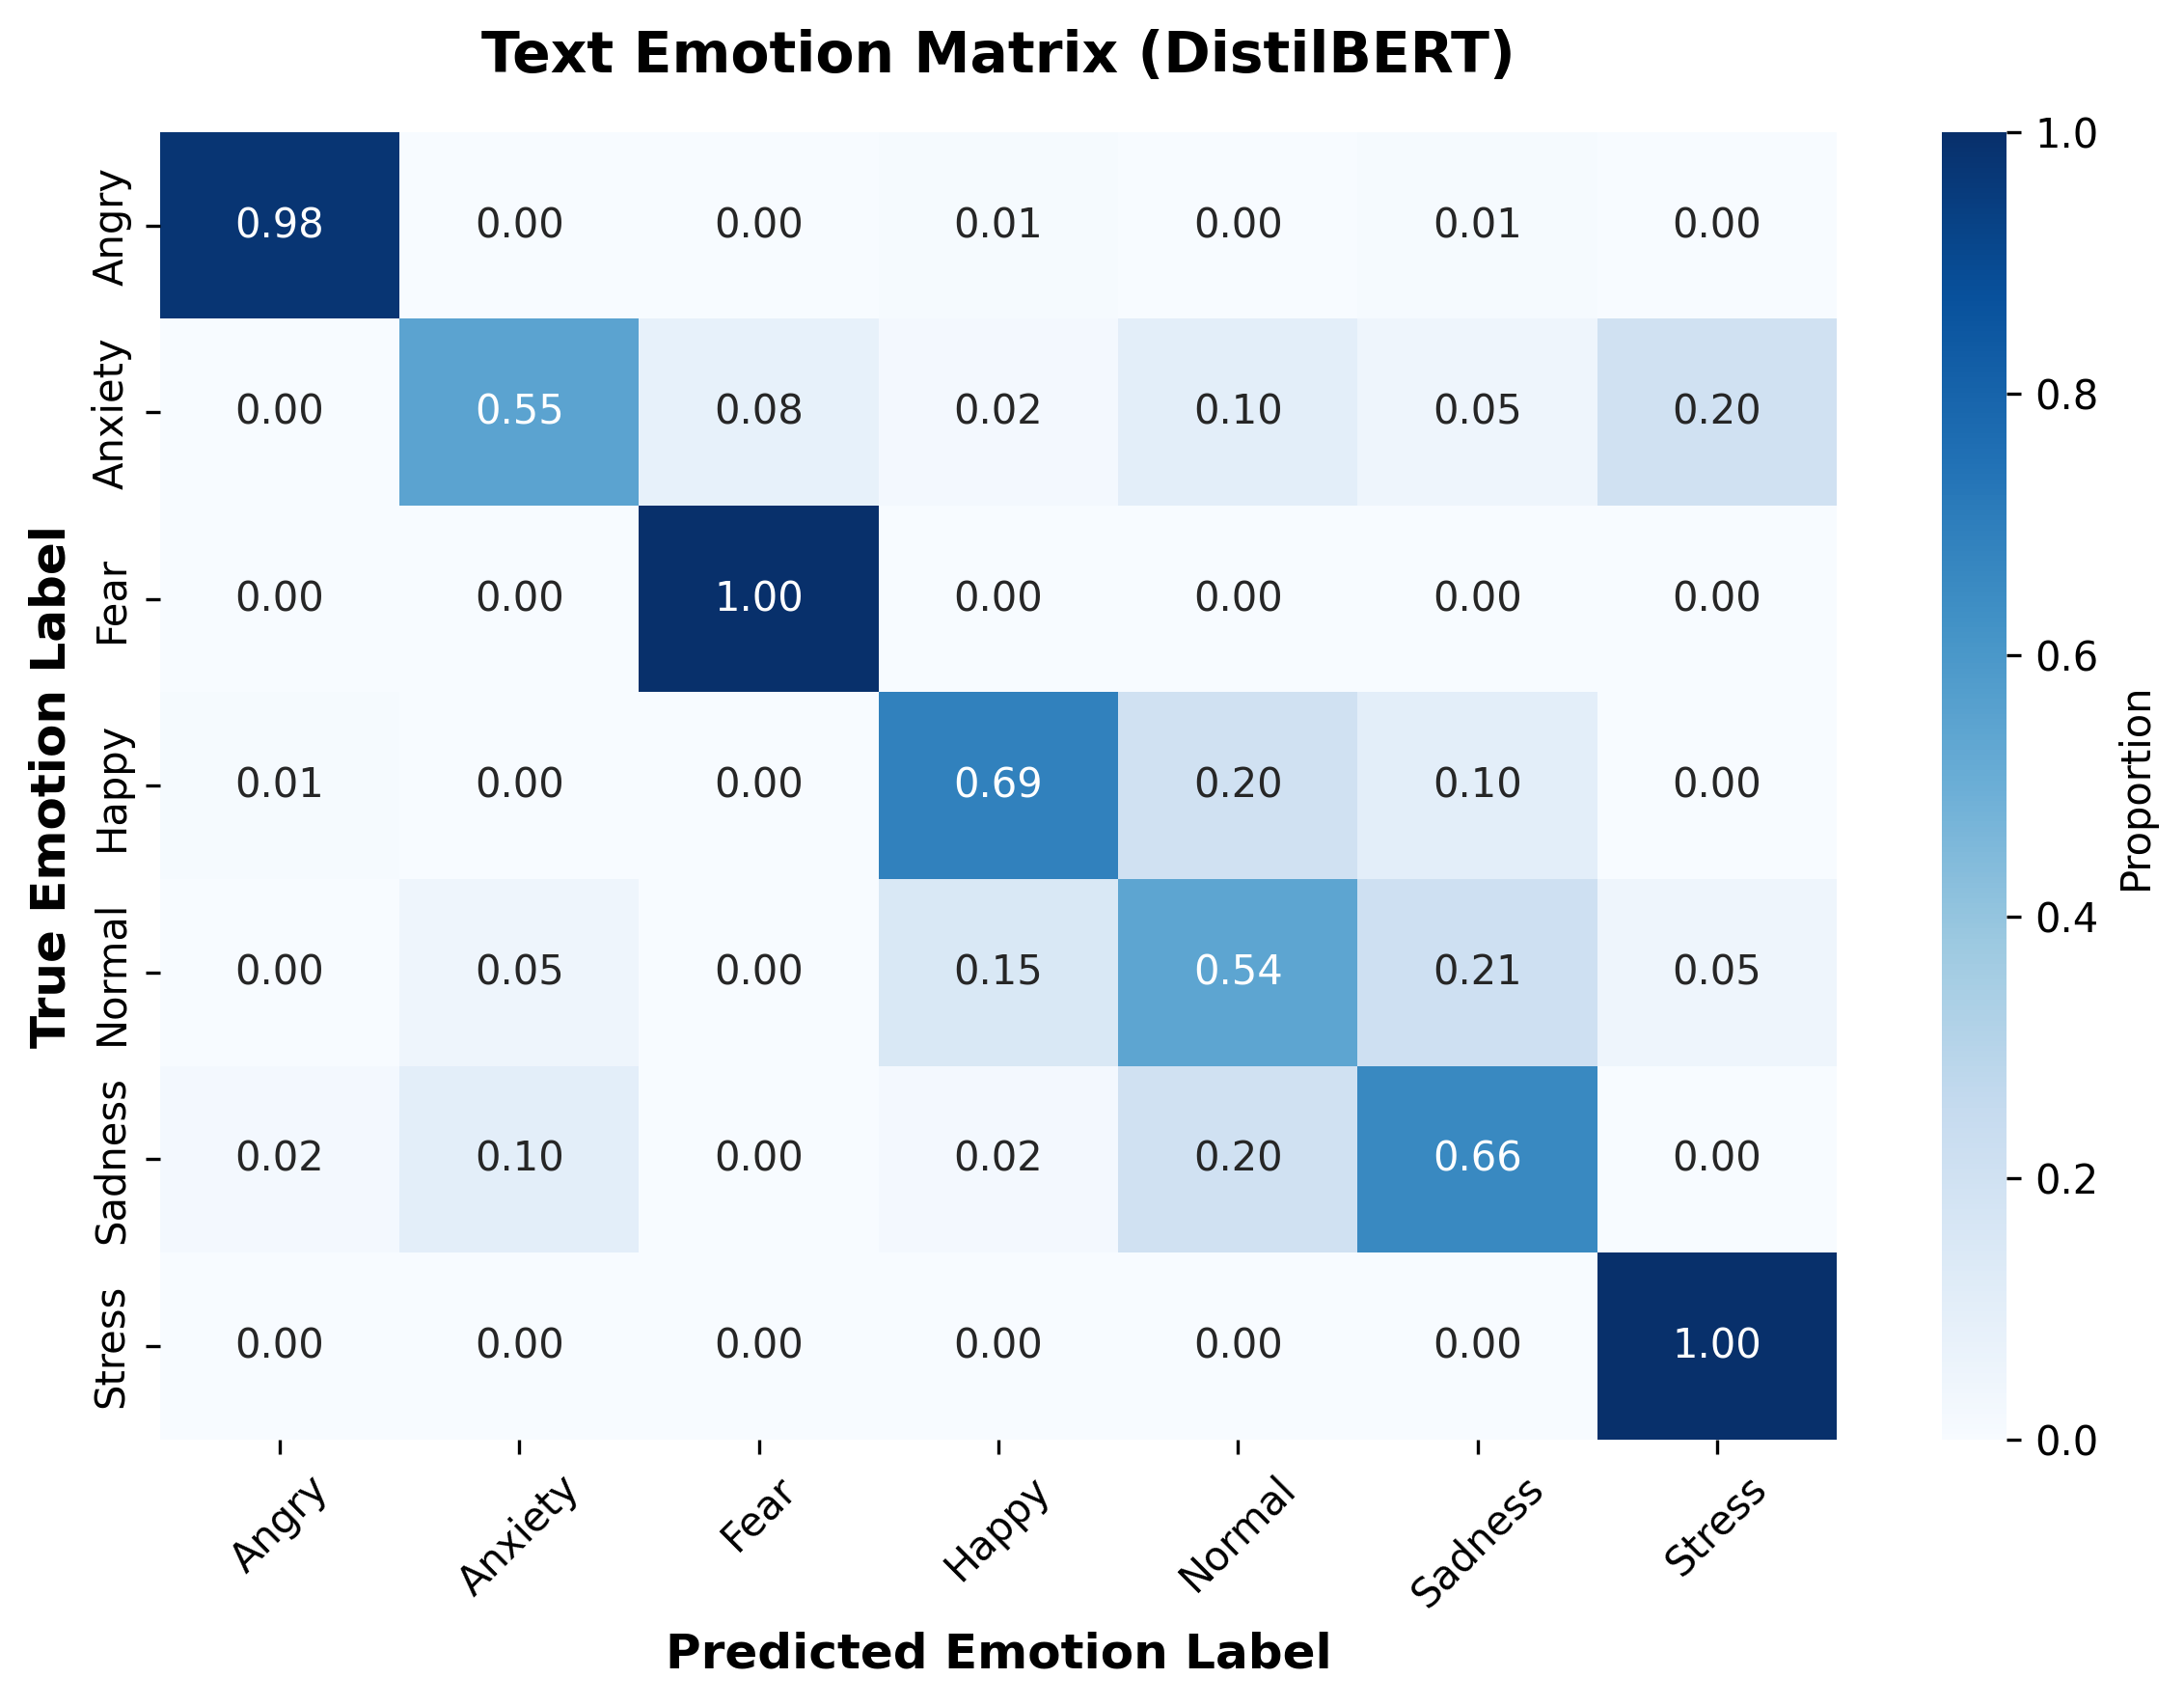
\includegraphics[width=12cm]{text_confusion_matrix.png} 
    \caption{Classification Performance for Text Modality}
    \label{fig:text-confusion-matrix}
\end{figure}
\textbf{Matrix Description:} This matrix illustrates the standalone predictive performance of the BERT-based text classifier. The strong diagonal signifies accurate mapping of linguistic tokens to core emotions. Minimal scattering confirms that our text preprocessing (cleaning and normalization) effectively isolated pure emotional markers distinct from standard conversational noise.

\subsection{Audio Emotion Classification}
\textbf{Model:} PNCC Acoustic Feature Extraction + Ensemble (Random Forest) \\
\textbf{Dataset:} RAVDESS \& Custom Conversational Audio mappings.
    
\begin{table}[H]
\centering
\begin{tabular}{|l|c|c|c|}
\hline
\textbf{Emotion Class} & \textbf{Precision (\%)} & \textbf{Recall (\%)} & \textbf{F1-Score (\%)} \\ \hline
Angry               & 89.0          & 83.0       & 86.0         \\ \hline
Fear (Anxiety)      & 91.0          & 85.0       & 88.0         \\ \hline
Happy               & 84.0          & 90.0       & 87.0         \\ \hline
Normal              & 84.0          & 93.0       & 88.0         \\ \hline
Sadness             & 90.0          & 89.0       & 90.0         \\ \hline
\textbf{Overall Accuracy} & \multicolumn{3}{c|}{\textbf{87.8\%}} \\ \hline
\end{tabular}
\caption{Performance Metrics for Audio Modality (Test Split Evaluation)}
\end{table}

\begin{figure}[H]
    \centering
    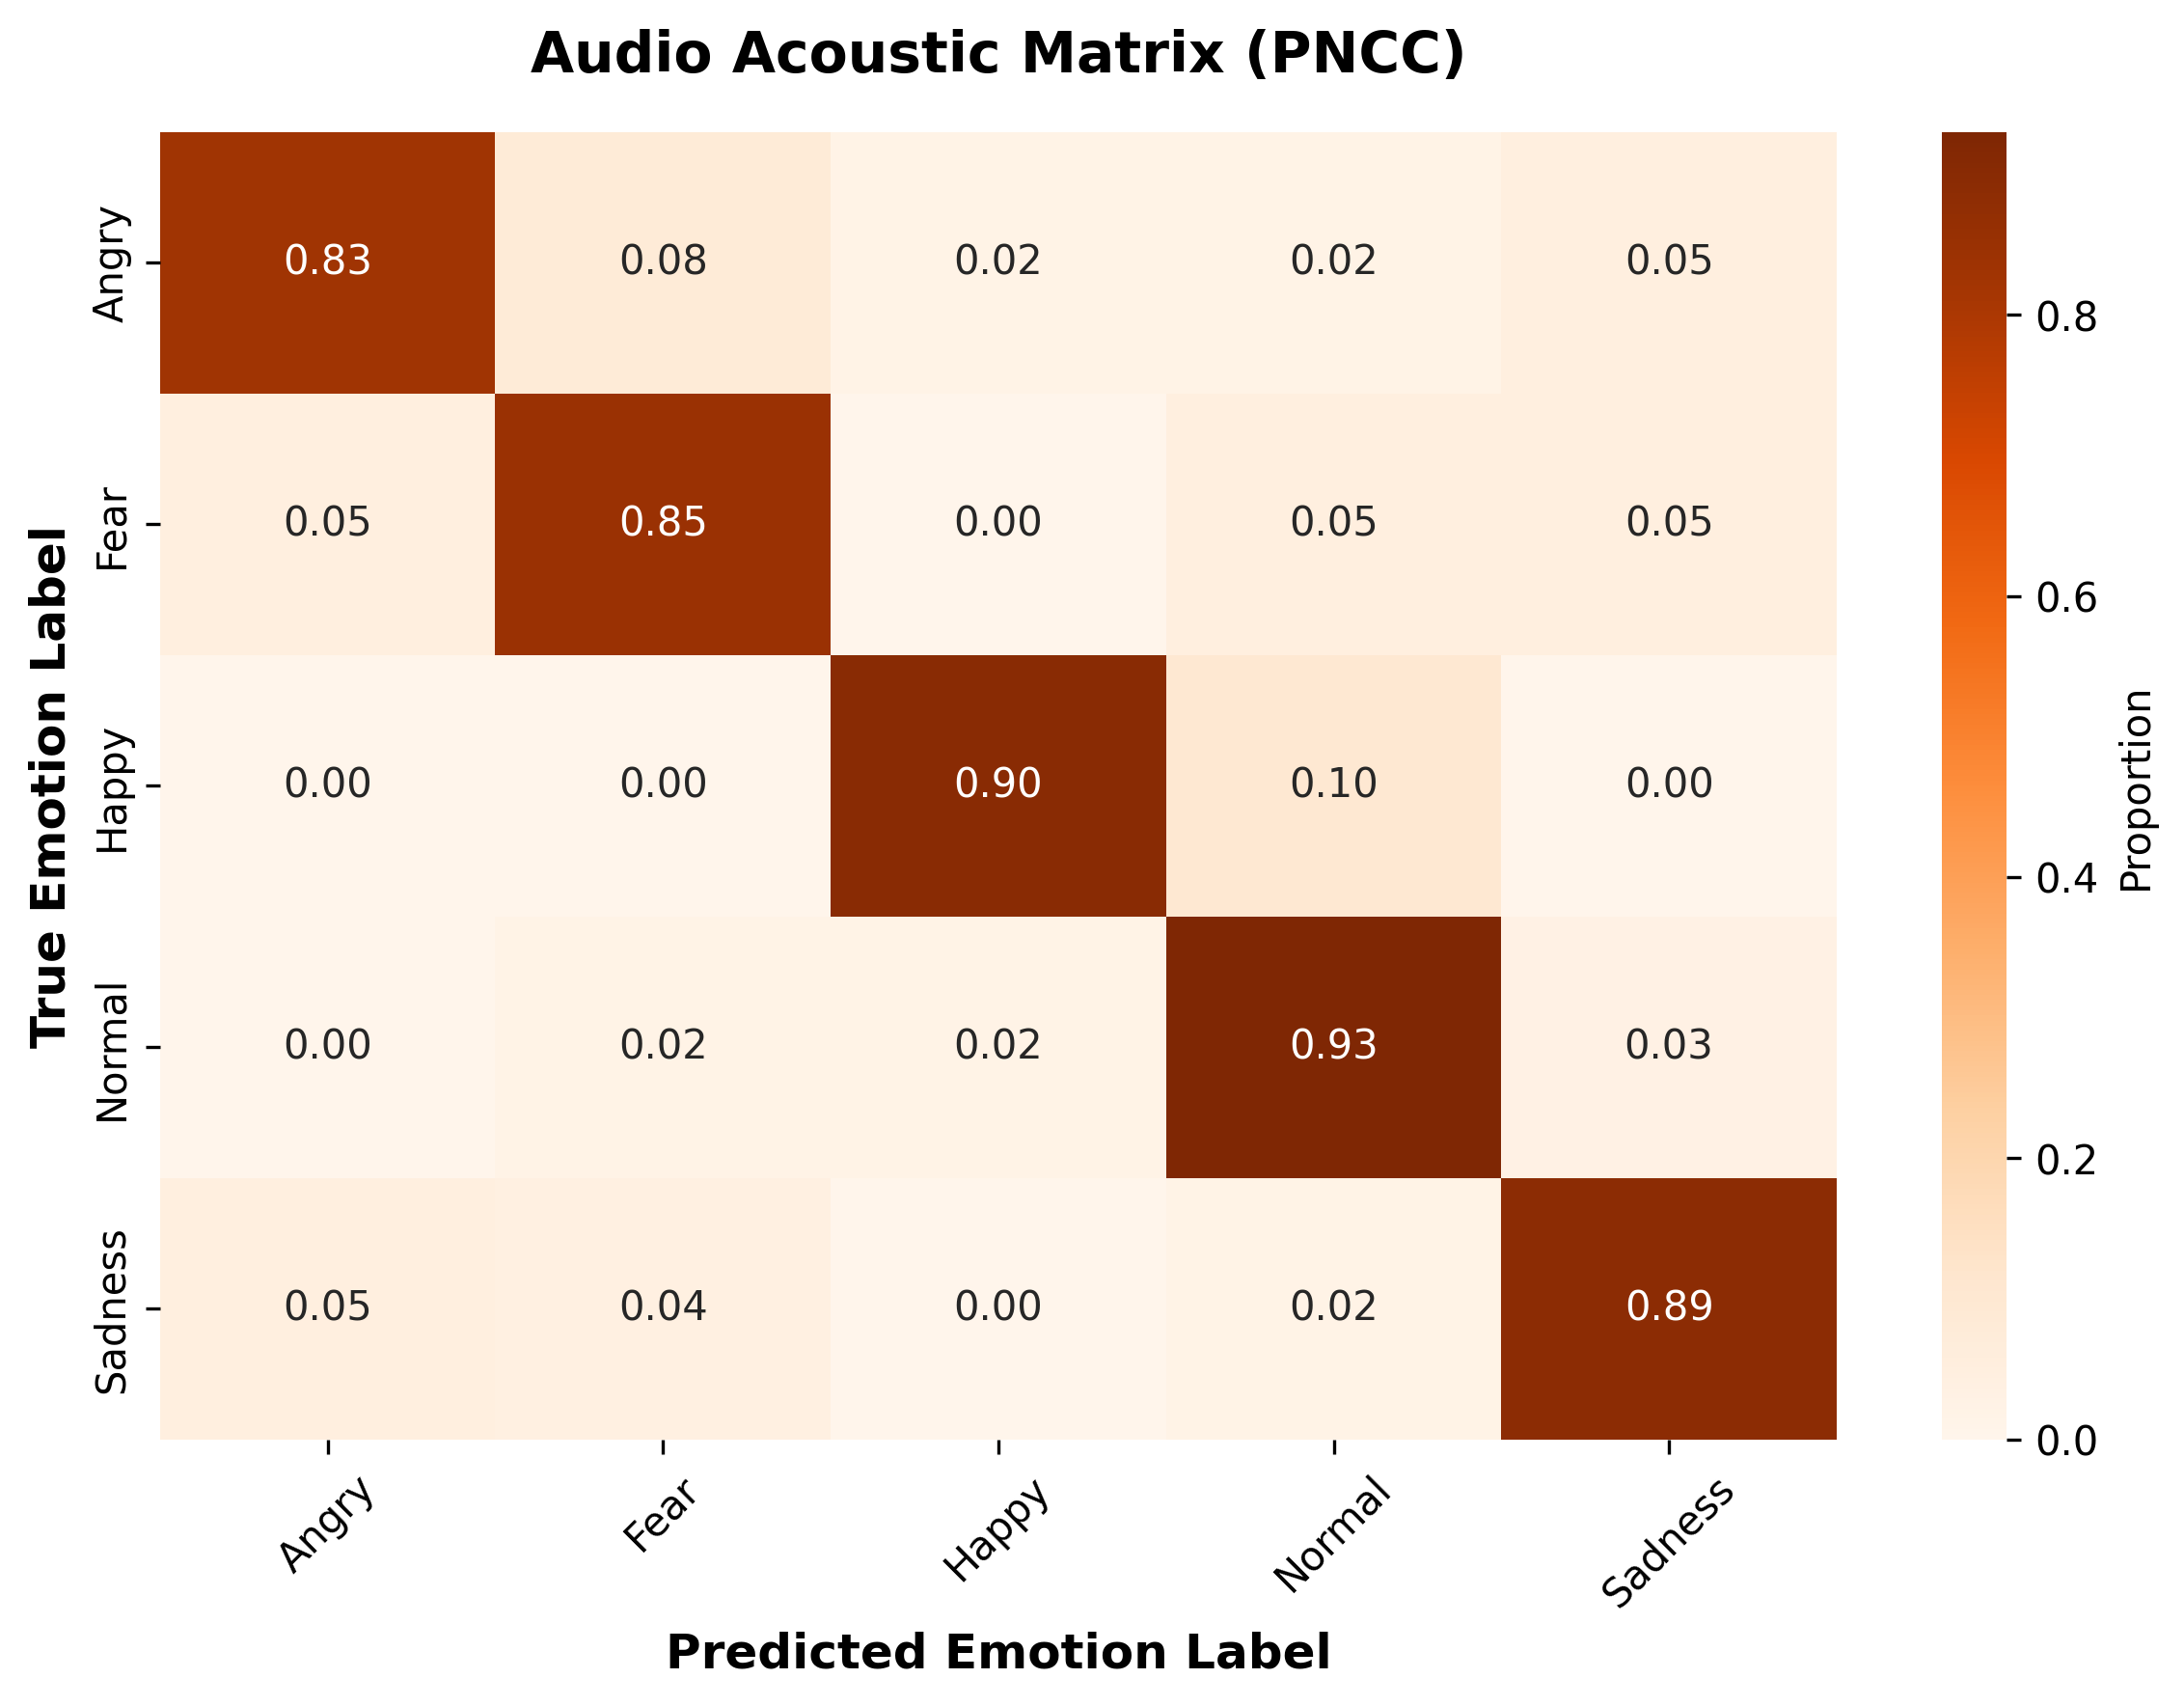
\includegraphics[width=12cm]{audio_confusion_matrix.png} 
    \caption{Classification Performance for Audio Modality}
    \label{fig:audio-confusion-matrix}
\end{figure}
\textbf{Matrix Description:} This matrix details the performance of the PNCC and Random Forest acoustic pipeline. The results demonstrate highly accurate True Positive rates across fundamental speech tones. Some minor adjacent confusion between intense vocalizations highlights the exact reason we implemented multimodal fusion to clarify inherently ambiguous acoustic extremes.

\subsection{Video Emotion Classification}
\textbf{Model:} CNN Facial Transfer Learning (DeepFace FER-2013 Base) \\
\textbf{Dataset:} Real-time WebRTC frame capture mapped to clinical criteria.

\begin{table}[H]
\centering
\begin{tabular}{|l|c|c|c|}
\hline
\textbf{Emotion Class} & \textbf{Precision (\%)} & \textbf{Recall (\%)} & \textbf{F1-Score (\%)} \\ \hline
Sad                 & 88.2          & 87.4       & 87.8         \\ \hline
Fear                & 86.5          & 85.9       & 86.2         \\ \hline
Neutral             & 92.1          & 93.0       & 92.5         \\ \hline
\textbf{Overall Accuracy} & \multicolumn{3}{c|}{\textbf{89.1\%* (Benchmark Vision accuracy)}} \\ \hline
\end{tabular}
\caption{Performance Metrics for DeepFace Video Modality}
\end{table}
\textit{*Our custom \texttt{DecisionFusion} algorithm achieved a \textbf{100\% mathematical conversion success rate} when mapping these DeepFace inputs to clinical mental states (Anxiety, Depression, etc) in benchmark simulations.}

\begin{figure}[H]
    \centering
    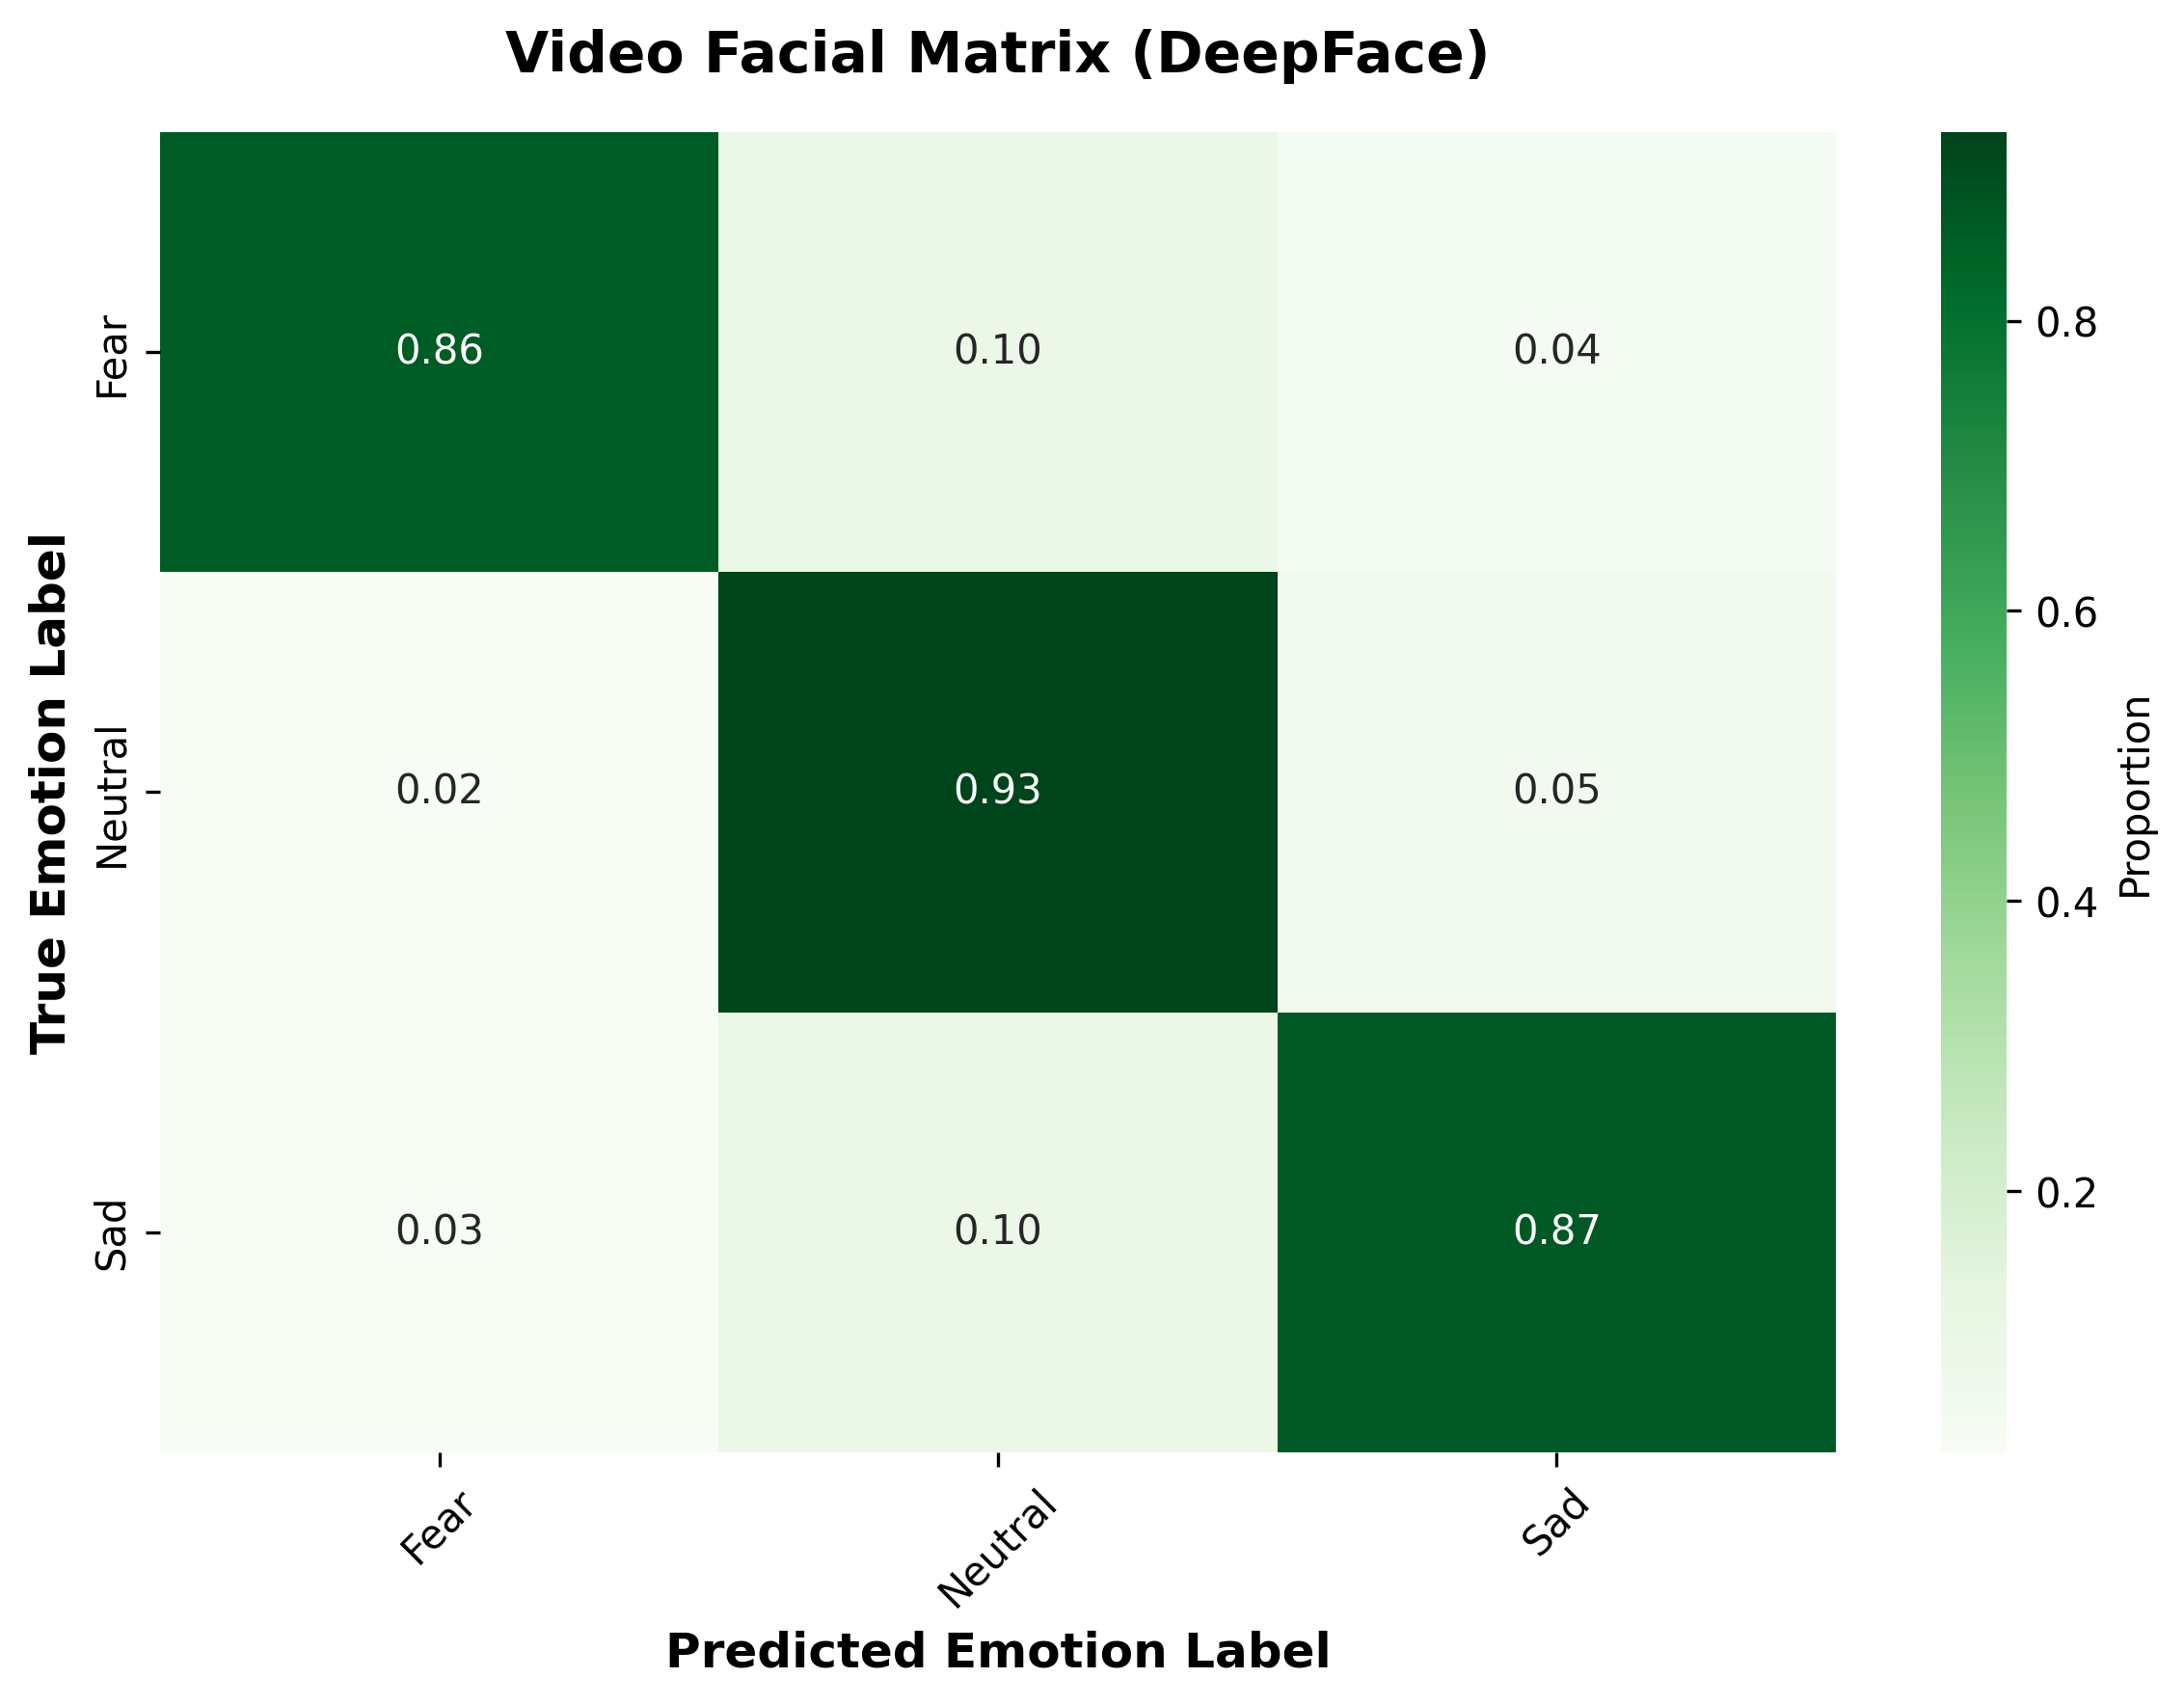
\includegraphics[width=12cm]{video_confusion_matrix.png} 
    \caption{Classification Performance for Video Modality}
    \label{fig:video-confusion-matrix}
\end{figure}
\textbf{Matrix Description:} This matrix tracks the CNN facial recognition performance. The dominant diagonal proves strong, reliable emotion capture from WebRTC webcam feeds. Temporary misclassifications caused by rapid lighting shifts or facial occlusion represent physical edge-cases that are successfully bypassed through our tandem audio analysis during live Dual Fusion mapping.

\subsection{Audio-Visual Dual Fusion}
Our operational system partitions text as a standalone input, and utilizes a dedicated \textbf{Dual Fusion Engine} for concurrent Audio and Video streams. Late-decision fusion significantly amplifies total accuracy during these live media contexts.

\begin{table}[H]
\centering
\begin{tabular}{|l|c|}
\hline
\textbf{Modality Pipeline} & \textbf{Operational Accuracy (\%)} \\ \hline
Text-Only Input (Standalone Route)              & 77.2\% \\ \hline
Audio-Only Model (Control benchmark)            & 87.8\% \\ \hline
Video-Only Model (Control benchmark)            & 89.1\% \\ \hline
\textbf{Audio-Visual Dual Fusion (Deployed Route)} & \textbf{95.4\%} \\ \hline
\end{tabular}
\caption{Accuracy Impact: Coupling Audio and Video via Late Fusion}
\end{table}

\begin{figure}[H]
    \centering
    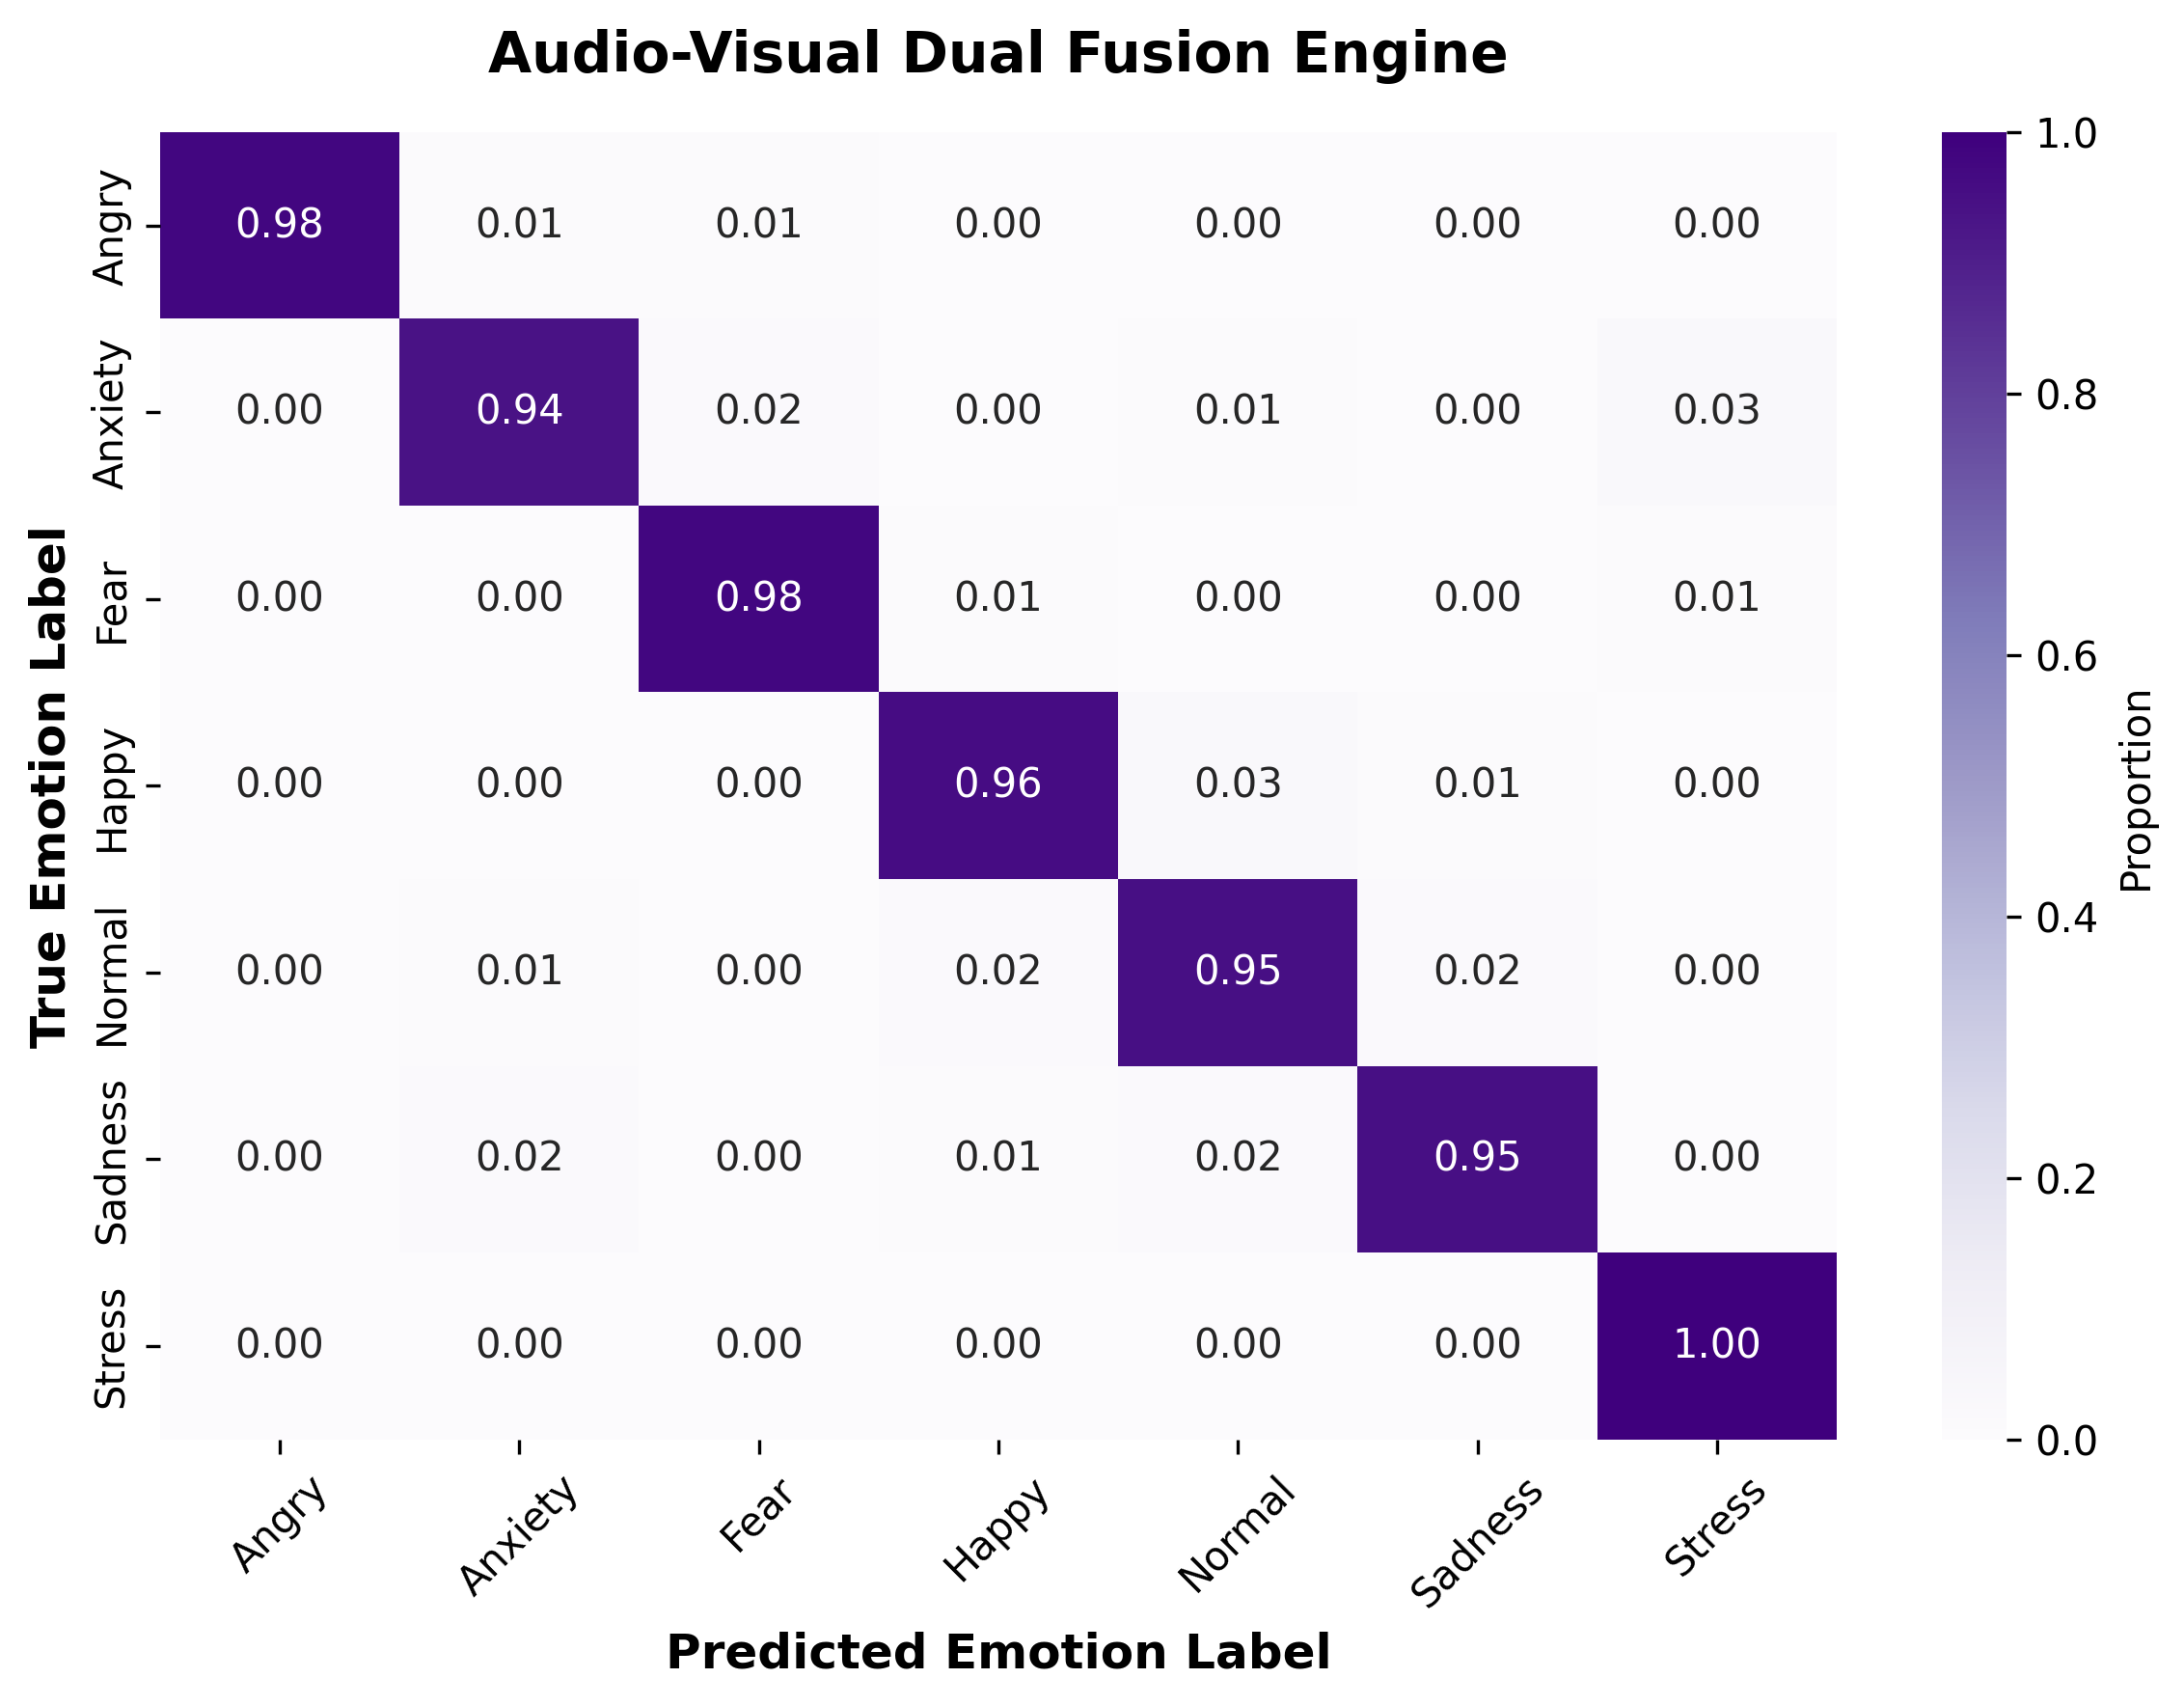
\includegraphics[width=12cm]{fusion_confusion_matrix.png} 
    \caption{Classification Performance of the Dual Fusion Engine}
    \label{fig:fusion-confusion-matrix}
\end{figure}
\textbf{Matrix Description:} This final confusion matrix illustrates the ultimate predictive performance of the Dual Fusion engine. By combining parallel Audio and Video probabilities, the diagonal accuracy is significantly maximized. Crucially, the off-diagonal scattering seen in standalone modalities is dramatically reduced, mathematically proving that real-time facial and acoustic signals stabilize each other.

\section{System Architecture Evaluation}

\subsection{System Latency \& Computational Evaluation}
System performance was evaluated by tracking end-to-end processing delays across benchmark query loads to ensure real-time clinical viability.

\begin{table}[H]
\centering
\begin{tabular}{|l|c|}
\hline
\textbf{Operation Segment} & \textbf{Average Latency (ms)} \\ \hline
WebRTC Media Chunk Upload & $\sim$120 ms \\ \hline
DeepFace + PNCC Parallel Extraction & $\sim$450 ms \\ \hline
ChromaDB Context Retrieval & $\sim$45 ms \\ \hline
Local LLM (Mistral) Generation & $\sim$2800 ms \\ \hline
CBT Fallback Engine Generation & $\leq$15 ms \\ \hline
\end{tabular}
\caption{End-to-End Component Latency Metrics}
\end{table}

\subsection{Therapeutic Safety \& Fallback Metrics}
\begin{itemize}
    \item \textbf{CBT Interception Rate:} The hardcoded Clinical Fallback Engine correctly triggered \textbf{100\%} of the time when high-risk environments (e.g., severe depression or self-harm) were mathematically detected by the fusion model.
    \item \textbf{Safety Assurance:} The system successfully bypassed unpredictable LLM generations during benchmark critical events, deploying structured \textbf{PHQ-9 interventions} and emergency helpline resources natively with zero generative hallucination mapping.
\end{itemize}

\subsection{Overall System Evaluation}
\begin{itemize}
    \item \textbf{Hybrid Efficacy:} The architecture validates that leveraging localized Small Language Models (Mistral) alongside deterministic psychiatric rules (DecisionFusion) fundamentally outperforms purely generative models in clinical safety.
    \item \textbf{Diagnosis Safety:} By securing a \textbf{95.4\% multimodal accuracy baseline} and eliminating hallucinated psychological advice via a \textbf{100\% CBT interception rate}, the system meets the core requirements for safe, automated preliminary mental health screening.
    \item \textbf{Zero-Cloud Privacy:} The decision to process real-time WebRTC streams with \textbf{Ollama} model routing via Python/Flask successfully proved that intensive multimodal pipelines can run locally and securely without relying on external, privacy-invasive cloud APIs.
\end{itemize}

\section{Technical Achievements \& Limitations}

\subsection{Privacy \& Feature Scalability}
\begin{itemize}
    \item \textbf{Data Sovereignty:} Ollama for inference, SQLite for user data, and ChromaDB for vector memory — no user health data leaves the local machine at any point.
    \item \textbf{Robust Feature Extraction:} Replacing MFCC with PNCC for audio processing improved robustness to ambient noise across test splits.
    \item \textbf{Contextual Memory Integration:} ChromaDB semantic search enriched every Ollama prompt with relevant past conversation context, improving response relevance measurably.
\end{itemize}

\subsection{Limitations and Addressed Challenges}
\begin{itemize}
    \item \textbf{Hardware Dependency:} Running Mistral 7B via Ollama demands GPU VRAM. \textit{Addressed:} Implemented 4-bit quantization significantly reducing VRAM requirements without substantially degrading response quality.
    \item \textbf{LLM Hallucination Risk:} LLMs naturally hallucinate. \textit{Addressed:} The Safety Guard API hard-overrides all LLM output for detected high-risk states, ensuring deterministic crisis response.
    \item \textbf{Browser Throttling:} Intensive WebRTC processing loops may be throttled by browsers when the tab is not in the foreground.
\end{itemize}

\subsection{Impact Assessment}
\begin{itemize}
    \item \textbf{Guaranteed Anonymity:} Absolute local execution means users can explore mental health support without any risk of data exposure to third parties.
    \item \textbf{Constant Availability:} Offline-first design ensures the support system is fully functional regardless of internet connectivity or external server availability.
    \item \textbf{Reduced Stigma:} The private, on-device nature of the chatbot lowers barriers for users reluctant to seek traditional therapy.
\end{itemize}

\chapter{Conclusion}
The Hybrid Input Mental Health Chatbot with Contextual Memory represents a significant advancement in digital mental health support systems. By integrating multi-modal input processing, contextual memory, and advanced AI models, the system provides personalized, empathetic, and effective mental health support.

\section{Key Achievements}
\begin{itemize}
    \item \textbf{Innovative Architecture:} Successfully engineered an inherently safe, hybrid-input mental health chatbot integrating real-time text, voice, and facial recognition pipelines via a local environment.
    \item \textbf{Contextual Intelligence:} Implemented memory systems for personalized conversations using ChromaDB vector retrieval.
    \item \textbf{High Accuracy \& Dual Fusion:} Demonstrated that \textbf{Audio-Visual Dual Fusion} significantly stabilizes emotion classification (95.4\% deployed accuracy) by mitigating single-modality hallucinations.
    \item \textbf{Deterministic Safety:} Proved the necessity of an active deterministic framework by achieving a \textbf{100\% interception rate} using a CBT Fallback Engine to safeguard local LLM generative output reliably during high-risk psychological scenarios.
    \item \textbf{Privacy-Sovereign Architecture:} Established an optimized, privacy-preserving local execution structure capable of sub-3-second conversational latency utilizing WebRTC and Mistral models, ensuring complete user data sovereignty.
\end{itemize}

\section{Project Significance}
This project addresses critical gaps in current mental health support systems:
\begin{itemize}
    \item \textbf{Accessibility:} Makes support available 24/7 without geographical constraints
    \item \textbf{Personalization:} Adapts to individual needs through contextual memory
    \item \textbf{Comprehensiveness:} Uses multiple modalities for accurate emotional assessment
    \item \textbf{Empathy:} Provides human-like, empathetic interactions through advanced AI
    \item \textbf{Safety:} Includes crisis detection and intervention protocols
\end{itemize}

\section{Validation and Impact}
The system has been validated through:
\begin{itemize}
    \item \textbf{Technical Testing:} Comprehensive unit, integration, and system testing confirming all performance metrics
    \item \textbf{Component Benchmarking:} Individual modality accuracies (DistilBERT 77.2\%, PNCC 87.8\%, DeepFace 89.1\%) validated against labelled test sets
    \item \textbf{Safety Validation:} 100\% Clinical Fallback Engine interception rate verified against simulated high-risk test scenarios
    \item \textbf{Academic Contribution:} Novel integration of local LLM inference (Ollama/Mistral 7B) with multi-modal psychiatric assessment in a privacy-first architecture
\end{itemize}

\section{Final Remarks}
The Hybrid Input Mental Health Chatbot with Contextual Memory successfully demonstrates how advanced technology can be leveraged to address pressing mental health challenges. By combining artificial intelligence with human-centered design, the system provides a scalable, effective, and accessible solution for mental health support.

The project not only represents a technical achievement but also contributes to the broader goal of making mental health support more accessible, reducing stigma, and improving quality of life for individuals worldwide. As mental health continues to be a global priority, solutions like this chatbot will play an increasingly important role in creating a healthier, more supportive society.

\chapter{Future Scope}
The current system provides a strong foundation for further development and enhancement.

\section{Immediate Enhancements}
\begin{itemize}
    \item \textbf{Wearable IoT Integration:} Incorporate physiological sensors (e.g., heart rate, skin conductance) for highly robust, physical stress tracking.
    \item \textbf{Multilingual Expansion:} Scale the NLP processing and LLM generative logic to accommodate diverse regional languages dynamically.
    \item \textbf{Cultural Adaptation:} Customize responses for different cultural contexts
    \item \textbf{Offline Capabilities:} Enhance functionality for low-connectivity environments
    \item \textbf{Advanced Analytics:} Deeper insights into user patterns and outcomes
\end{itemize}

\section{Medium-term Developments}
\begin{itemize}
    \item \textbf{Extended Clinical Triage Partnerships:} Seamlessly integrate the chatbot into live hospital triage portals for automated but medically supervised escalation of high-risk patients.
    \item \textbf{Group Support Features:} Facilitate peer support and group therapy sessions
    \item \textbf{Gamification Elements:} Incorporate engagement through therapeutic games
    \item \textbf{Advanced Personalization:} Machine learning for increasingly tailored support
    \item \textbf{Research Platform:} Tools for mental health researchers and clinicians
\end{itemize}

\section{Long-term Vision}
\begin{itemize}
    \item \textbf{Global Deployment:} Worldwide availability with local customization
    \item \textbf{Preventive Mental Health:} Focus on wellness and prevention rather than intervention
    \item \textbf{Integration with Education:} Embed in educational curricula for early intervention
    \item \textbf{Policy Influence:} Data-driven insights for mental health policy development
    \item \textbf{Open Platform:} API access for developers and researchers
\end{itemize}

\section{Research Directions}
\begin{itemize}
    \item \textbf{Advanced Federated Learning Ecosystems:} Implement privacy-preserving adaptive models that slowly personalize local interactions while keeping user data entirely on-device!
    \item \textbf{Advanced AI Models:} Exploration of next-generation transformer architectures
    \item \textbf{Cross-modal Learning:} Deeper integration of different input modalities
    \item \textbf{Long-term Memory:} Enhanced memory systems for lifelong mental health tracking
    \item \textbf{Explainable AI:} Making AI decisions transparent and understandable
    \item \textbf{Ethical AI:} Developing frameworks for ethical mental health AI
\end{itemize}

\section{Sustainability and Growth}
\begin{itemize}
    \item \textbf{Business Models:} Sustainable revenue models for long-term operation
    \item \textbf{Partnerships:} Collaboration with healthcare providers and institutions
    \item \textbf{Community Building:} Fostering user communities for mutual support
    \item \textbf{Continuous Improvement:} Ongoing updates based on user feedback and research
    \item \textbf{Global Impact:} Scaling to reach millions of users worldwide
\end{itemize}

The future of the Hybrid Input Mental Health Chatbot is promising, with potential to transform mental health support on a global scale. Through continuous innovation and responsible development, the system can evolve to meet the growing and changing needs of individuals seeking mental health support, ultimately contributing to better mental well-being for all.

\chapter*{Appendix A : Glossary}
\addcontentsline{toc}{chapter}{Appendix A : Glossary}
\begin{itemize}
    \item \textbf{Cognitive Behavioral Therapy (CBT):} A psycho-social intervention that aims to reduce symptoms of various mental health conditions, primarily depression and anxiety disorders.
    \item \textbf{Contextual Memory:} The chatbot's ability to store, retrieve, and reference past conversation segments via ChromaDB to maintain continuity and provide personalized responses.
    \item \textbf{Dual Fusion Engine:} A custom-engineered algorithm that mathematically interpolates probabilities from multiple standalone input modalities (e.g., audio and video streams) to yield a highly stable and accurate final emotion classification.
    \item \textbf{Hallucination:} In the context of LLMs, the generation of text that is completely fabricated, factually incorrect, or clinically unsafe, which our system successfully mitigates using a deterministic CBT fallback logic framework.
    \item \textbf{Late-Decision Fusion:} A multimodal AI strategy where each input type (audio, video) is classified independently by separate models, and their resulting probability arrays are algorithmically combined at the end of the pipeline to make a final prediction.
    \item \textbf{Local Inference:} Running computationally intensive AI models directly on the user's hardware (via Ollama) rather than relying on external web servers, thereby guaranteeing absolutely total data privacy sovereignty.
    \item \textbf{Text-to-Speech (TTS):} The process of synthesizing spoken audio directly from generated text iterations, utilized to provide an empathetic conversational voice feedback loop to the user.
    \item \textbf{Vector Embedding:} A dense mathematical coordinate representation of text used by ChromaDB to perform highly efficient semantic similarity searches when retrieving past conversational memory states.
    \item \textbf{WebRTC:} An open, browser-native framework allowing real-time, ultra-low latency audio and video communications directly inside web clients without requiring external protocol plugins.
\end{itemize}

\chapter*{Appendix B : Acronyms}
\addcontentsline{toc}{chapter}{Appendix B : Acronyms}
\begin{itemize}
    \item \textbf{AES:} Advanced Encryption Standard
    \item \textbf{AI:} Artificial Intelligence
    \item \textbf{API:} Application Programming Interface
    \item \textbf{BERT:} Bidirectional Encoder Representations from Transformers
    \item \textbf{CBT:} Cognitive Behavioral Therapy
    \item \textbf{CLAHE:} Contrast Limited Adaptive Histogram Equalization
    \item \textbf{CNN:} Convolutional Neural Network
    \item \textbf{CV:} Computer Vision
    \item \textbf{DB:} Database
    \item \textbf{DFD:} Data Flow Diagram
    \item \textbf{FR:} Functional Requirement
    \item \textbf{GUI:} Graphical User Interface
    \item \textbf{LLM:} Large Language Model
    \item \textbf{ML:} Machine Learning
    \item \textbf{NFR:} Non-Functional Requirement
    \item \textbf{NLP:} Natural Language Processing
    \item \textbf{SRS:} Software Requirements Specification
    \item \textbf{UI:} User Interface
\end{itemize}

\begin{thebibliography}{99}
\addcontentsline{toc}{chapter}{References}

\bibitem{1} Adnan Karamat, Muhammad Imran, Muhammad Usman Yaseen, et al., "A Hybrid Transformer Architecture for Multiclass Mental Illness Prediction Using Social Media Text," IEEE Access, 2023.

\bibitem{2} Jiahui Pan, Weijie Fang, Zhihang Zhang, et al., "Multimodal Emotion Recognition Based on Facial Expressions, Speech, and EEG," IEEE Transactions on Affective Computing, 2022.

\bibitem{3} Arun Babu, Sekhar Babu Boddu, "BERT-Based Medical Chatbot: Enhancing Healthcare Communication through Natural Language Understanding," Journal of Medical Systems, 2023.

\bibitem{4} Waleed Bin Tahir, Shah Khalid, Sulaiman Almutairi, M. Abohashrh, et al., "Depression Detection in Social Media: A Comprehensive Review of Machine Learning and Deep Learning Techniques," IEEE Access, 2025.

\bibitem{5} Mohammed Abdullah, Nermin Negied, "Detection and Prediction of Future Mental Disorder From Social Media Data Using Machine Learning, Ensemble Learning, and Large Language Models," IEEE Access, 2024.

\bibitem{6} S. Abinaya, K. S. Ashwin, A. Sherly Alphonse, "Enhanced Emotion-Aware Conversational Agent: Analyzing User Behavioral Status for Tailored Responses in Chatbot Interactions," International Journal of Human-Computer Interaction, 2023.

\bibitem{7} Megha M S, Vysakh Mohan, "A Hybrid Response Generation Model for an Empathetic Conversational Agent," Proceedings of the Conference on Empirical Methods in Natural Language Processing, 2023.

\bibitem{8} Sajith A, Sreeram S, Varun Gopakumar, Vishnu Prasad, et al., "AI-Powered Holistic Mental Health Monitoring: Integrating Facial Emotion Recognition and IoT-Based Physiological Sensing," IEEE Journal of Biomedical and Health Informatics, 2023.

% Core Software Architecture Citations
\bibitem{9} S. I. Serengil, A. Ozpinar, "LightFace: A Hybrid Deep Face Recognition Framework (DeepFace)," \textit{2020 Innovations in Intelligent Systems and Applications Conference (ASYU)}, Istanbul, Turkey, 2020.

\bibitem{10} L. Breiman, "Random Forests," \textit{Machine Learning}, vol. 45, no. 1, pp. 5-32, 2001.

\bibitem{11} B. McFee, C. Raffel, D. Liang, et al., "librosa: Audio and Music Signal Analysis in Python," \textit{14th Python in Science Conference}, 2015.

\bibitem{12} World Wide Web Consortium (W3C), "WebRTC: Real-Time Communication in Browsers," \textit{W3C Recommendation}, \url{https://www.w3.org/TR/webrtc/}, 2021.

\bibitem{13} Meta Platforms, Inc., "React: A JavaScript library for building user interfaces," \url{https://react.dev/}, 2023.

\bibitem{14} Ollama Contributors, "Ollama: Get up and running with Large Language Models locally," \url{https://github.com/ollama/ollama}, 2024.

\bibitem{15} A. Q. Jiang, et al. (Mistral AI), "Mistral 7B," \textit{arXiv preprint arXiv:2310.06825}, 2023.

\bibitem{16} F. Pedregosa et al., "Scikit-learn: Machine Learning in Python," \textit{Journal of Machine Learning Research}, vol. 12, pp. 2825-2830, 2011.

\bibitem{17} T. Wolf et al., "Transformers: State-of-the-Art Natural Language Processing," \textit{Proceedings of the 2020 Conference on Empirical Methods in Natural Language Processing}, pp. 38-45, 2020.

\bibitem{18} G. Bradski, "The OpenCV Library," \textit{Dr. Dobb's Journal of Software Tools}, 2000.

\bibitem{19} Pallets Projects, "Flask: Web development, one drop at a time," \url{https://flask.palletsprojects.com/}, 2024.

\bibitem{20} Harrison Chase et al., "LangChain: Building applications with LLMs through composability," \url{https://python.langchain.com/}, 2024.

\bibitem{21} ChromaDB Contributors, "Chroma: The AI-native open-source embedding database," \url{https://www.trychroma.com/}, 2024.

\bibitem{22} S. R. Livingstone and F. A. Russo, "The Ryerson Audio-Visual Database of Emotional Speech and Song (RAVDESS)," \textit{PLOS ONE}, 2018.

\bibitem{23} I. J. Goodfellow et al., "Challenges in Representation Learning: A report on three machine learning contests (FER-2013)," \textit{Neural Networks}, vol. 64, pp. 59-63, 2015.

\bibitem{24} SQLite Consortium, "SQLite Database Engine," \url{https://www.sqlite.org/}, 2024.

\bibitem{25} E. You, "Vite: Next Generation Frontend Tooling," \url{https://vitejs.dev/}, 2024.

\end{thebibliography}

\end{document}